\subsubsection{Logistic map (LOG)} \label{subsubsec:log}

Logistic map is interesting because is representative of the very large family of quadratic maps.
Its expression is:
\begin{equation}\label{eq:logimap}
 x_{[n+1]}=4x_{[n]}(1-x_{[n]}) \,
\end{equation}
with $x_n\in\mathcal{R}$.

Note that to effectively work in a given representation it is necessary to change the expression of the map in order to make all the operations in the chosen representation numbers. For example, in the case of LOG the expression in binary fixed point numbers is:
\begin{equation}\label{eq:logimapB2}
x_{n+1}=4 \epsilon floor\{\frac{x_n(1-x_n)}{\epsilon}\} \,
\end{equation}
with $\epsilon = 2^B$ where $B$ is the number of bits that represents the fractional part.

According as B grows, statistical properties vary until they stabilize.
Figs. \ref{fig:LOG_QuantiB} (a) to (f) show the statistical properties of LOG map in floating point and fixed point representation.
All these figures show: $100$ red points for each fixed point precision ($B$) and in black their average (dashed black line connecting black dots), $100$ horizontal dashed blue lines that are the results of each run in floating point and a black solid line their average.
In this case, all the lines of the floating point are overlapped.

For $B\geq 30$ the value of $H_{val}$ remains almost identical to the values for the floating point representation whereas $H_{BP}$ and $C_{BP}$ stabilizes at $B>21$.
Their values are: $<H_{val}>=0.9669$; $<H_{BP}>=0.6269$; $<C_{BP}>=0.4843$.
Note that the stable value of missing patterns $MP=645$ makes the optimum $H_{BP} \leq ln(75)/ln(720) \simeq 0.65$.
Then, $B=30$ is the most convenient choice because an increase in the number of fractional digits does not improve the statistical properties.

Some conclusions can be drawn regarding \textit{BP} and \textit{BPW} quantifiers.
For $B=1, 2, 3$ and $4$, the averaged $BP$ quantifiers are almost $0$ while the averaged $BPW$ quantifiers can not be calculated (seein Figs. \ref{fig:LOG_QuantiB} c and e the missing black dashed line).
For those sequences where the initial condition where $0$ all iterations result to be a sequence of $0$s (the fixed point of the map), this happens very likely with small precisions because of the roundoffs.

When $B$ increases, $B=7, 9$ and $12$, the used initial conditions are rounded to zero less frequently.
So the generated sequences start from some value but many of them fall to zero with a short transitory.
This can be seen in Figs. c and e, $BPW$ shows high dispersion unlike $BP$ quantifiers.
This is because $BPW$ procedure takes into account only the transient discarding fixed points, unlike $BP$ procedure that considers all the sequence. 
 
\textcolor{red}{ESTE PÁRRAFO VA A DESAPARECER CON LONG DOUBLE, O NO?, ADEMÁS DISTRAE DEL FOCO DEL TRABAJO. HAY QUE BUSCARLE UN LUGAR EN EL PAPER}
Finally, for $B = 45, 49, 51$ and $52$ some $BP$ quantifiers have a low value, but $BPW$ quantifiers have a more predictible behavior, we can see that these atractors fall to a fixed point with a long transitory.
In this behaviour is due to the employed plataform.
The operation miltiplication needs the double of bits to be represented but the machine has only $64$.
Acá lo que quiero decir es que en las figuras \ref{fig:LOG_QuantiB} a, b y d las corridas con punto fijo tienen alta dispersión y aparecen algunas con valores muy bajos.
Esto es por que la aritmética de punto fijo la estamos queriendo generar artificialmente con una variable de tipo double que tiene una mantisa de 53 bits.
Entonces en la multiplicación (que duplica la cantidad de bits necesarios) se pierden muchos fraccionarios.
Lo mismo pasa si se usa el tipo float, que tiene 27 bits de mantisa pero mucho antes, a partir de B>24+-.
Con long double debería desaparecer.
Entonces hay que tener en cuenta esto cuando se simula punto fijo con la computadora, en los mapas que halla multiplicaciones.

\begin{figure}
	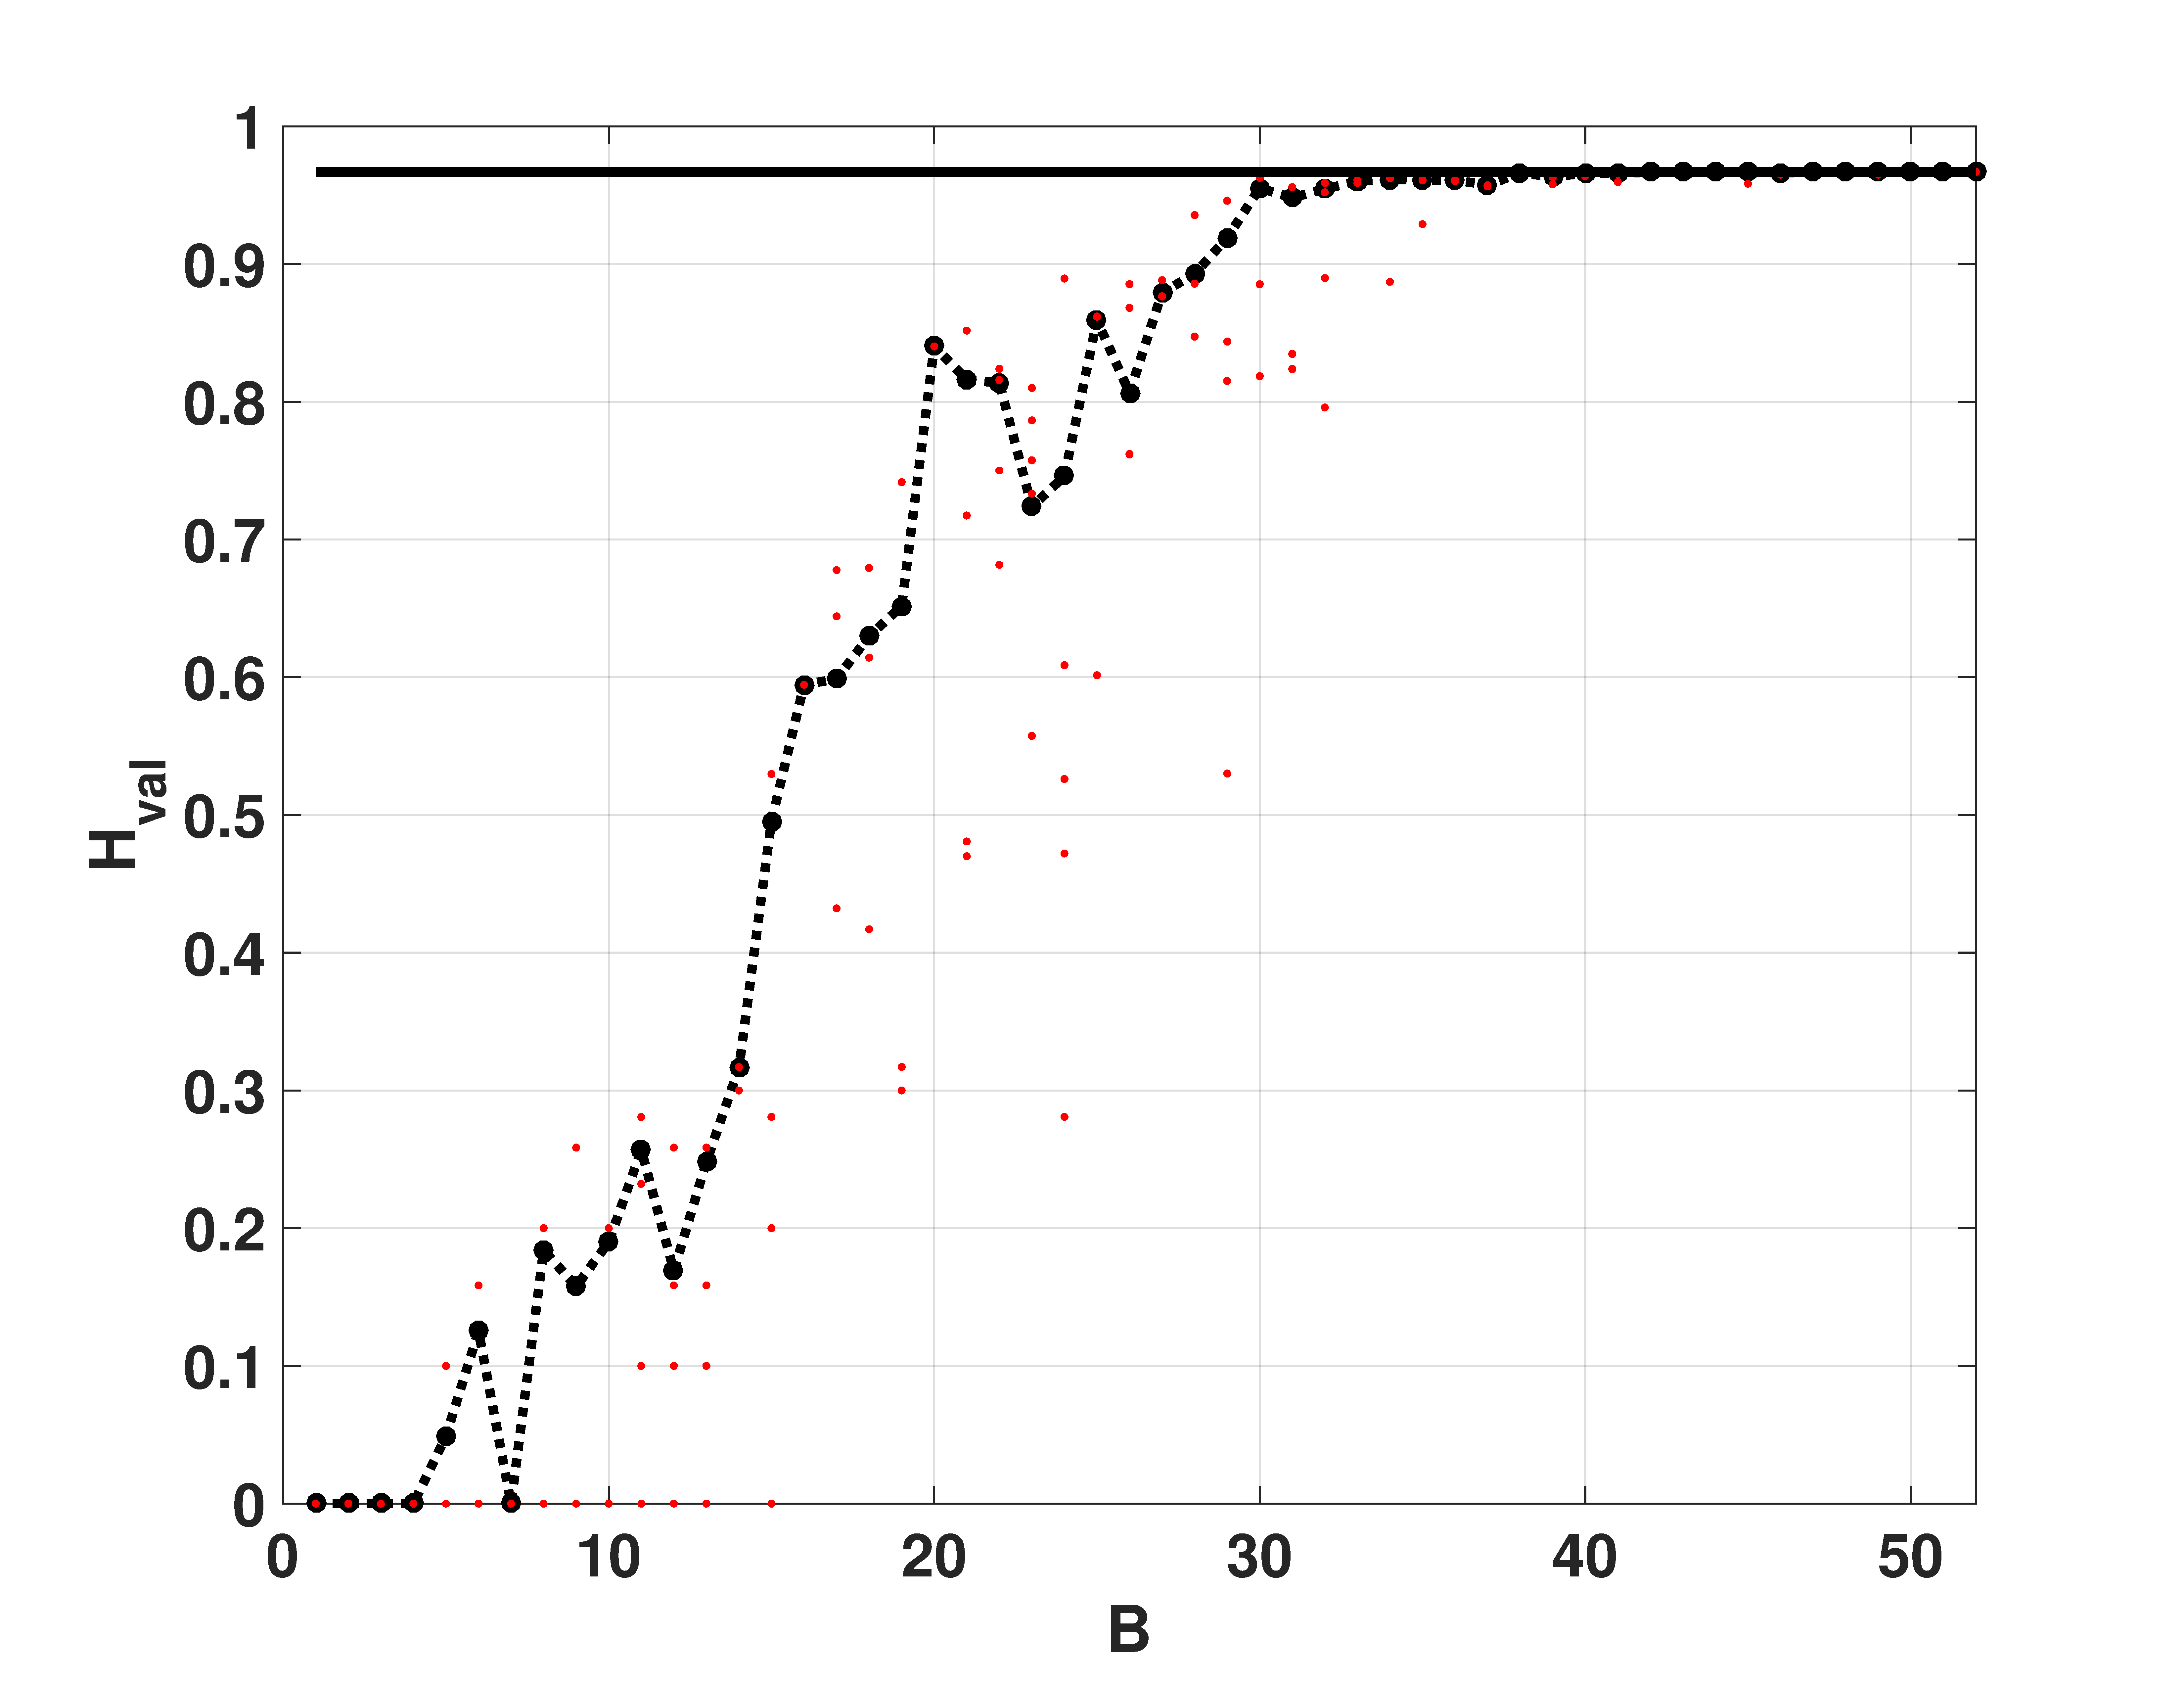
\includegraphics[width= .49\textwidth]{Hval_Log}
	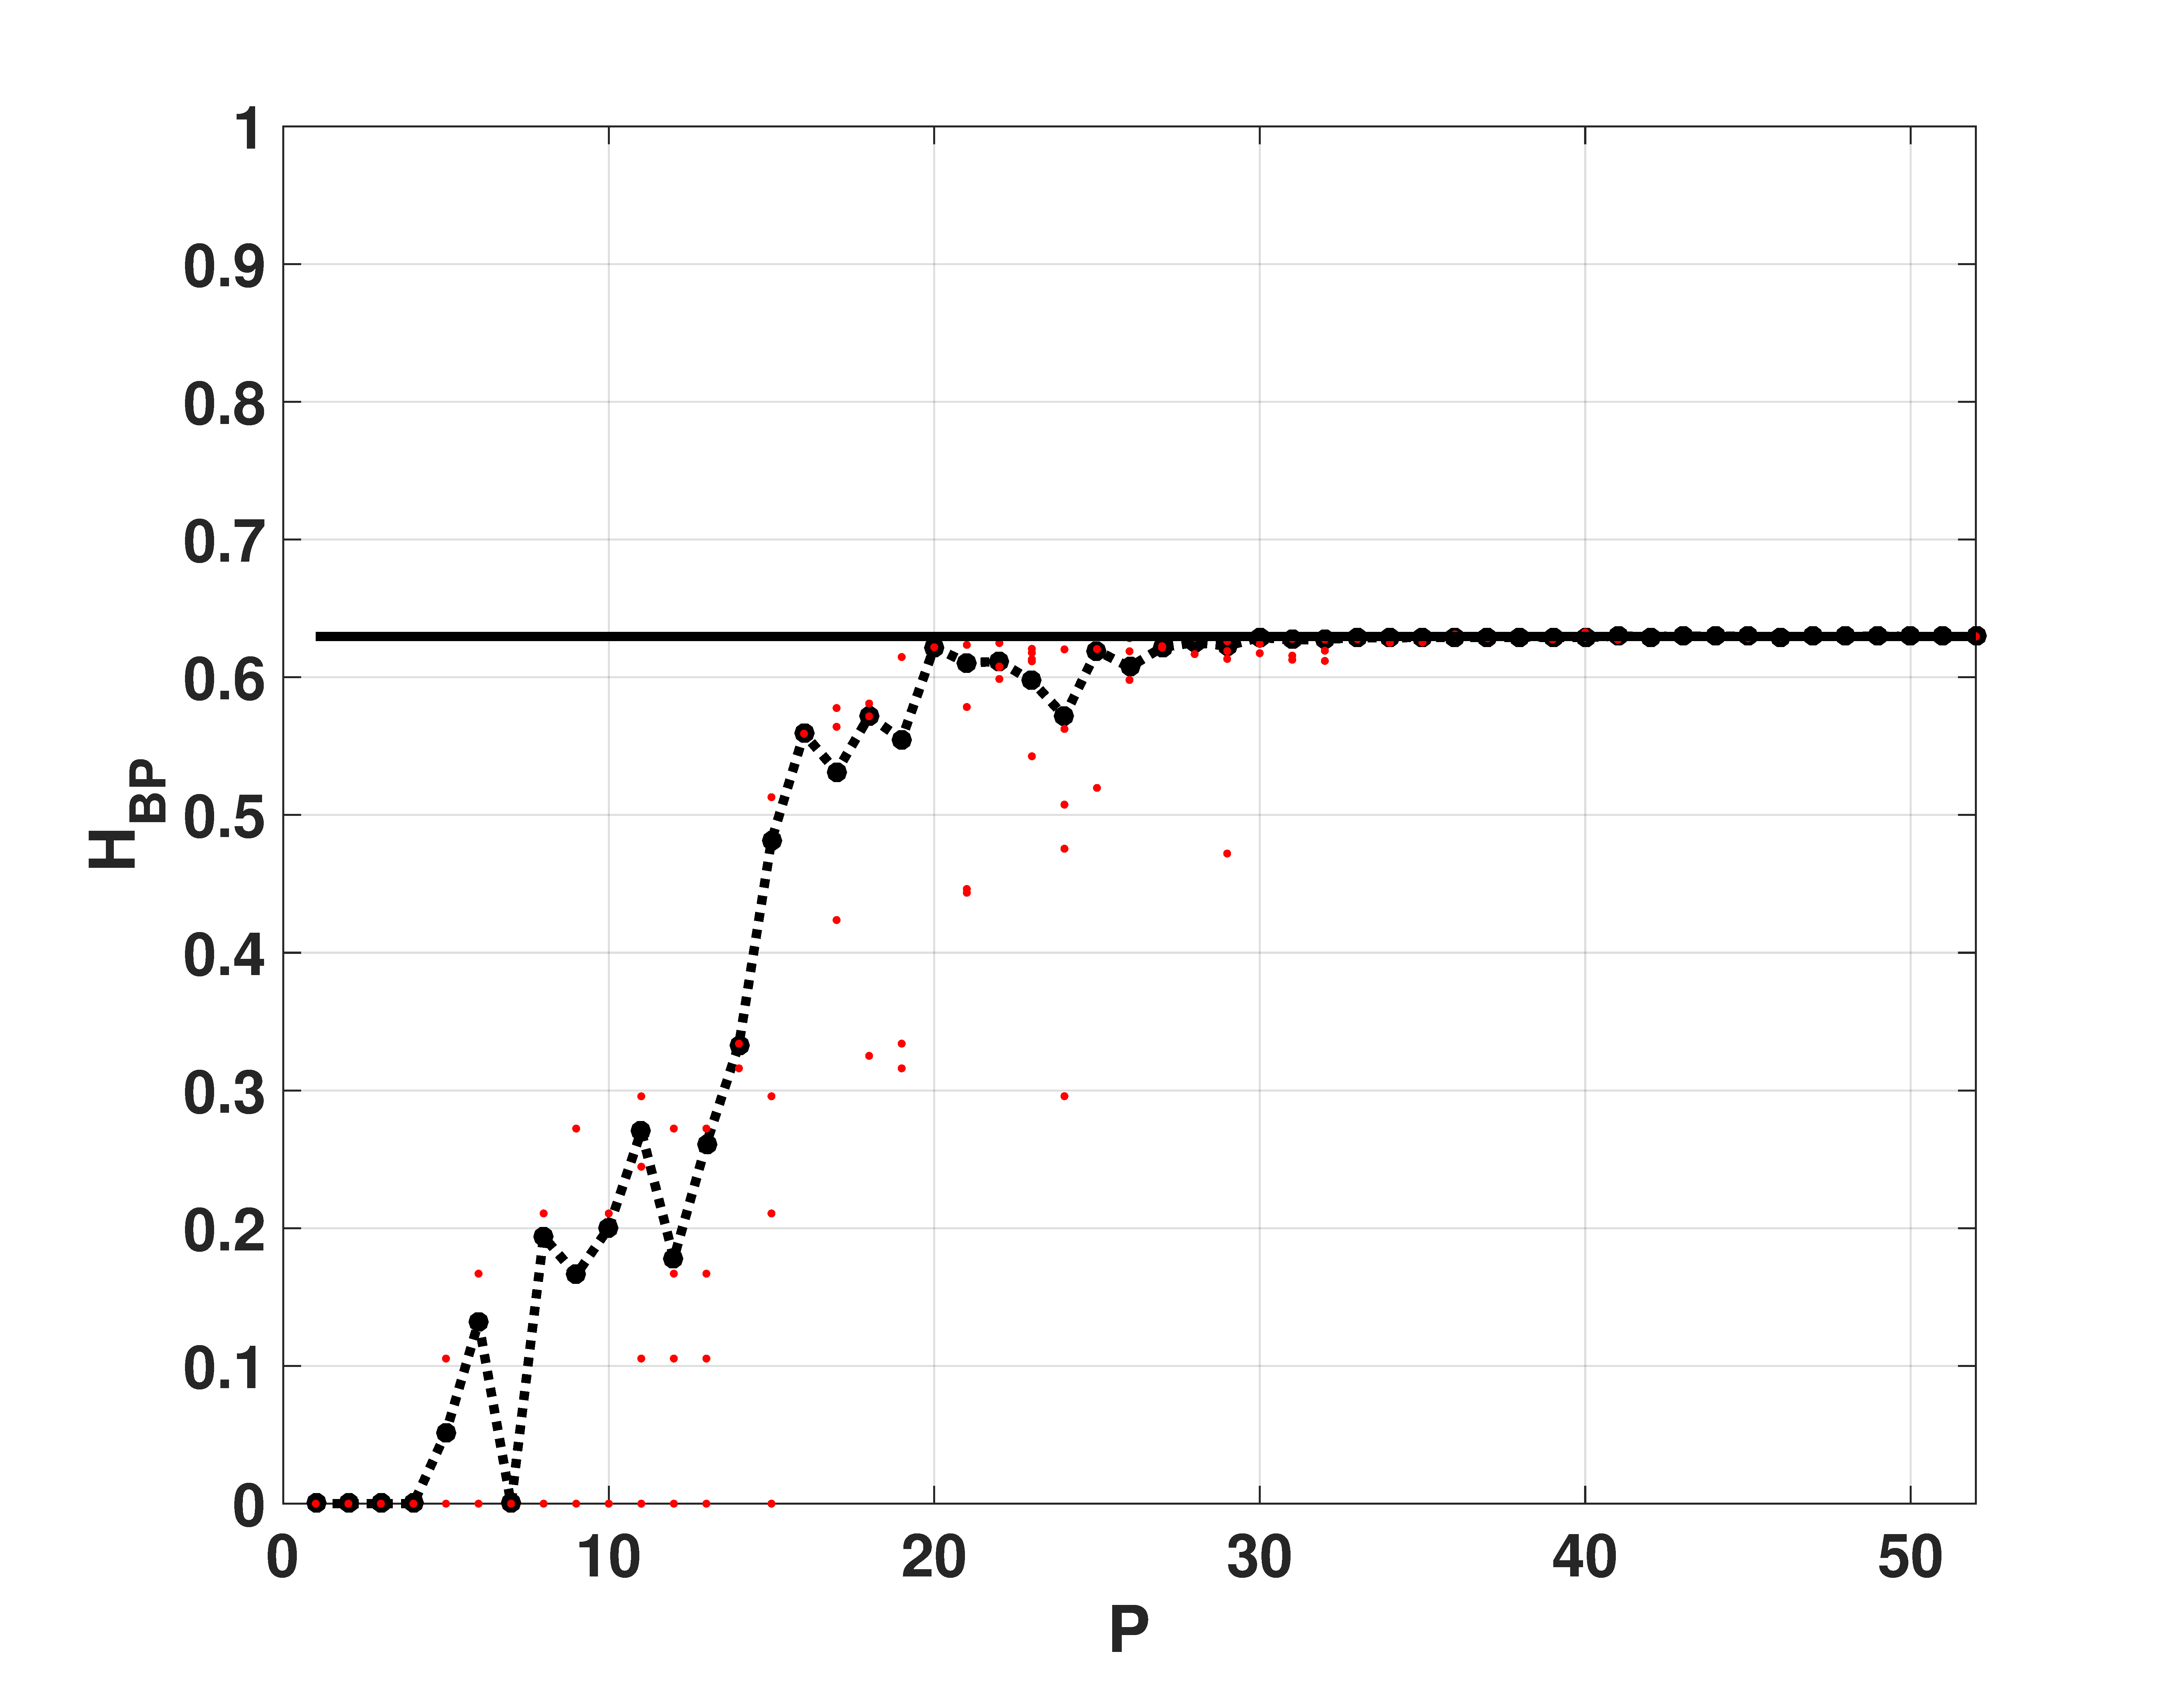
\includegraphics[width= .49\textwidth]{Hbp_Log}
	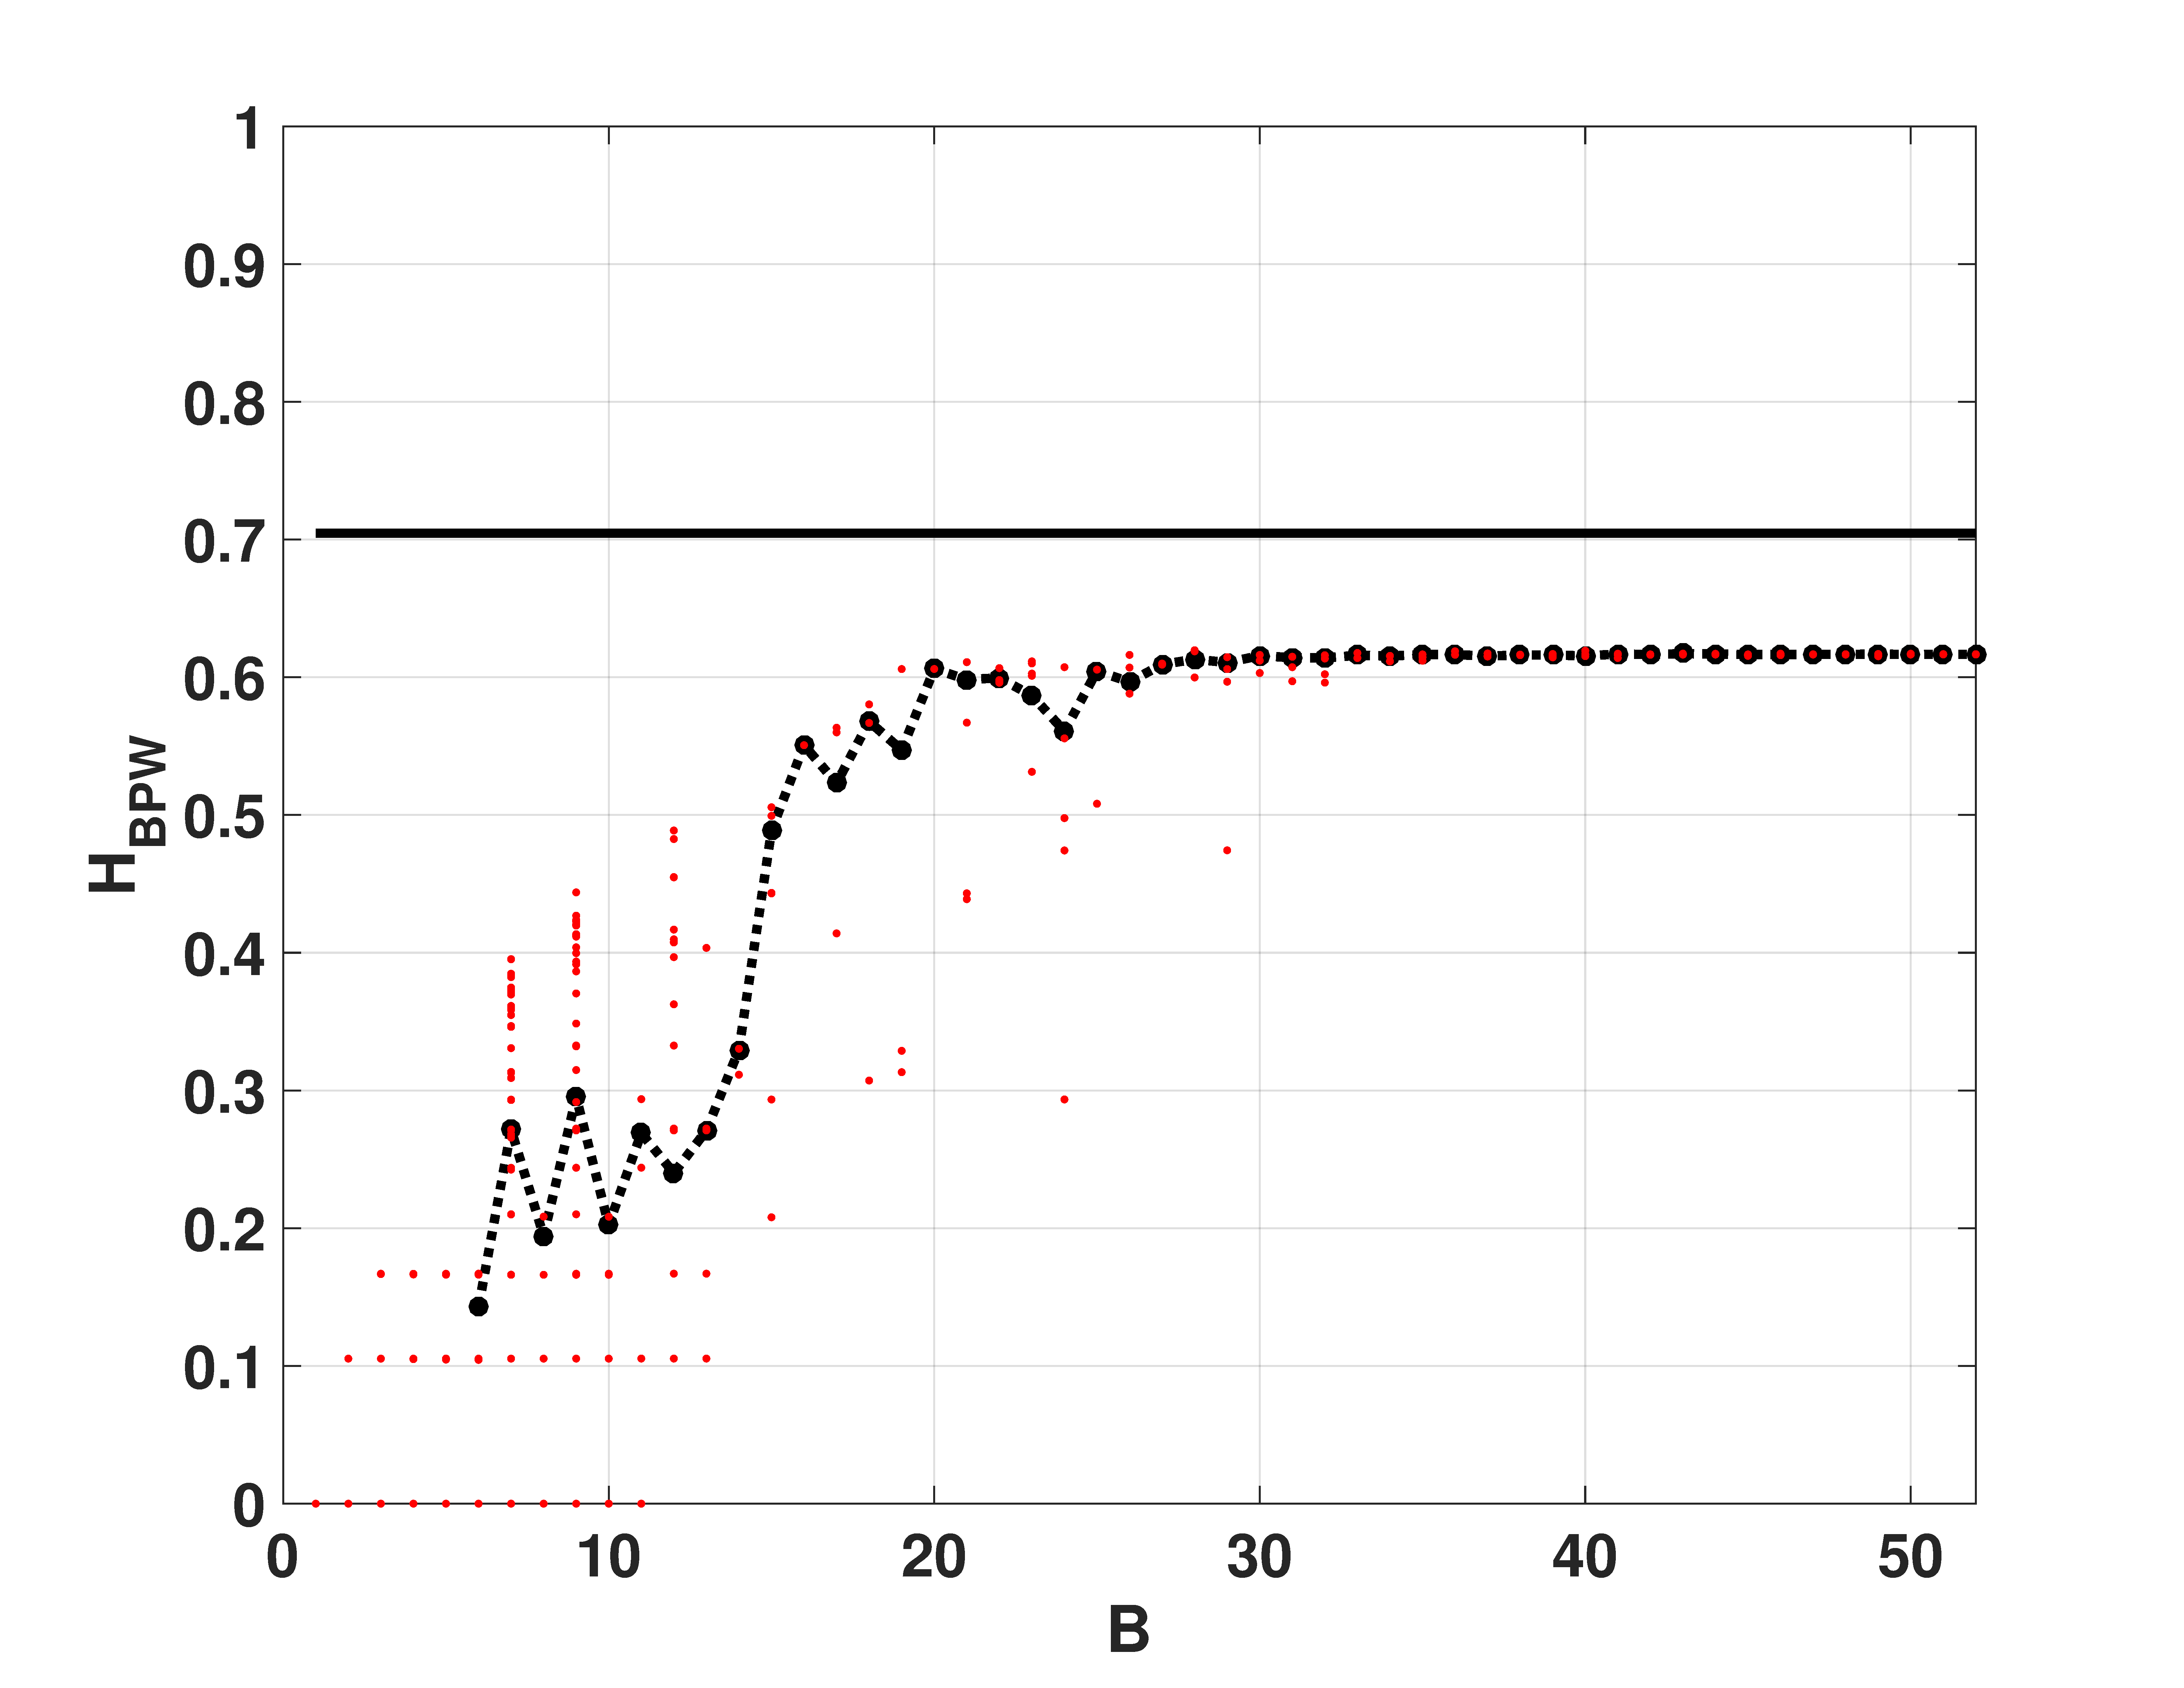
\includegraphics[width= .49\textwidth]{Hbpw_Log}
	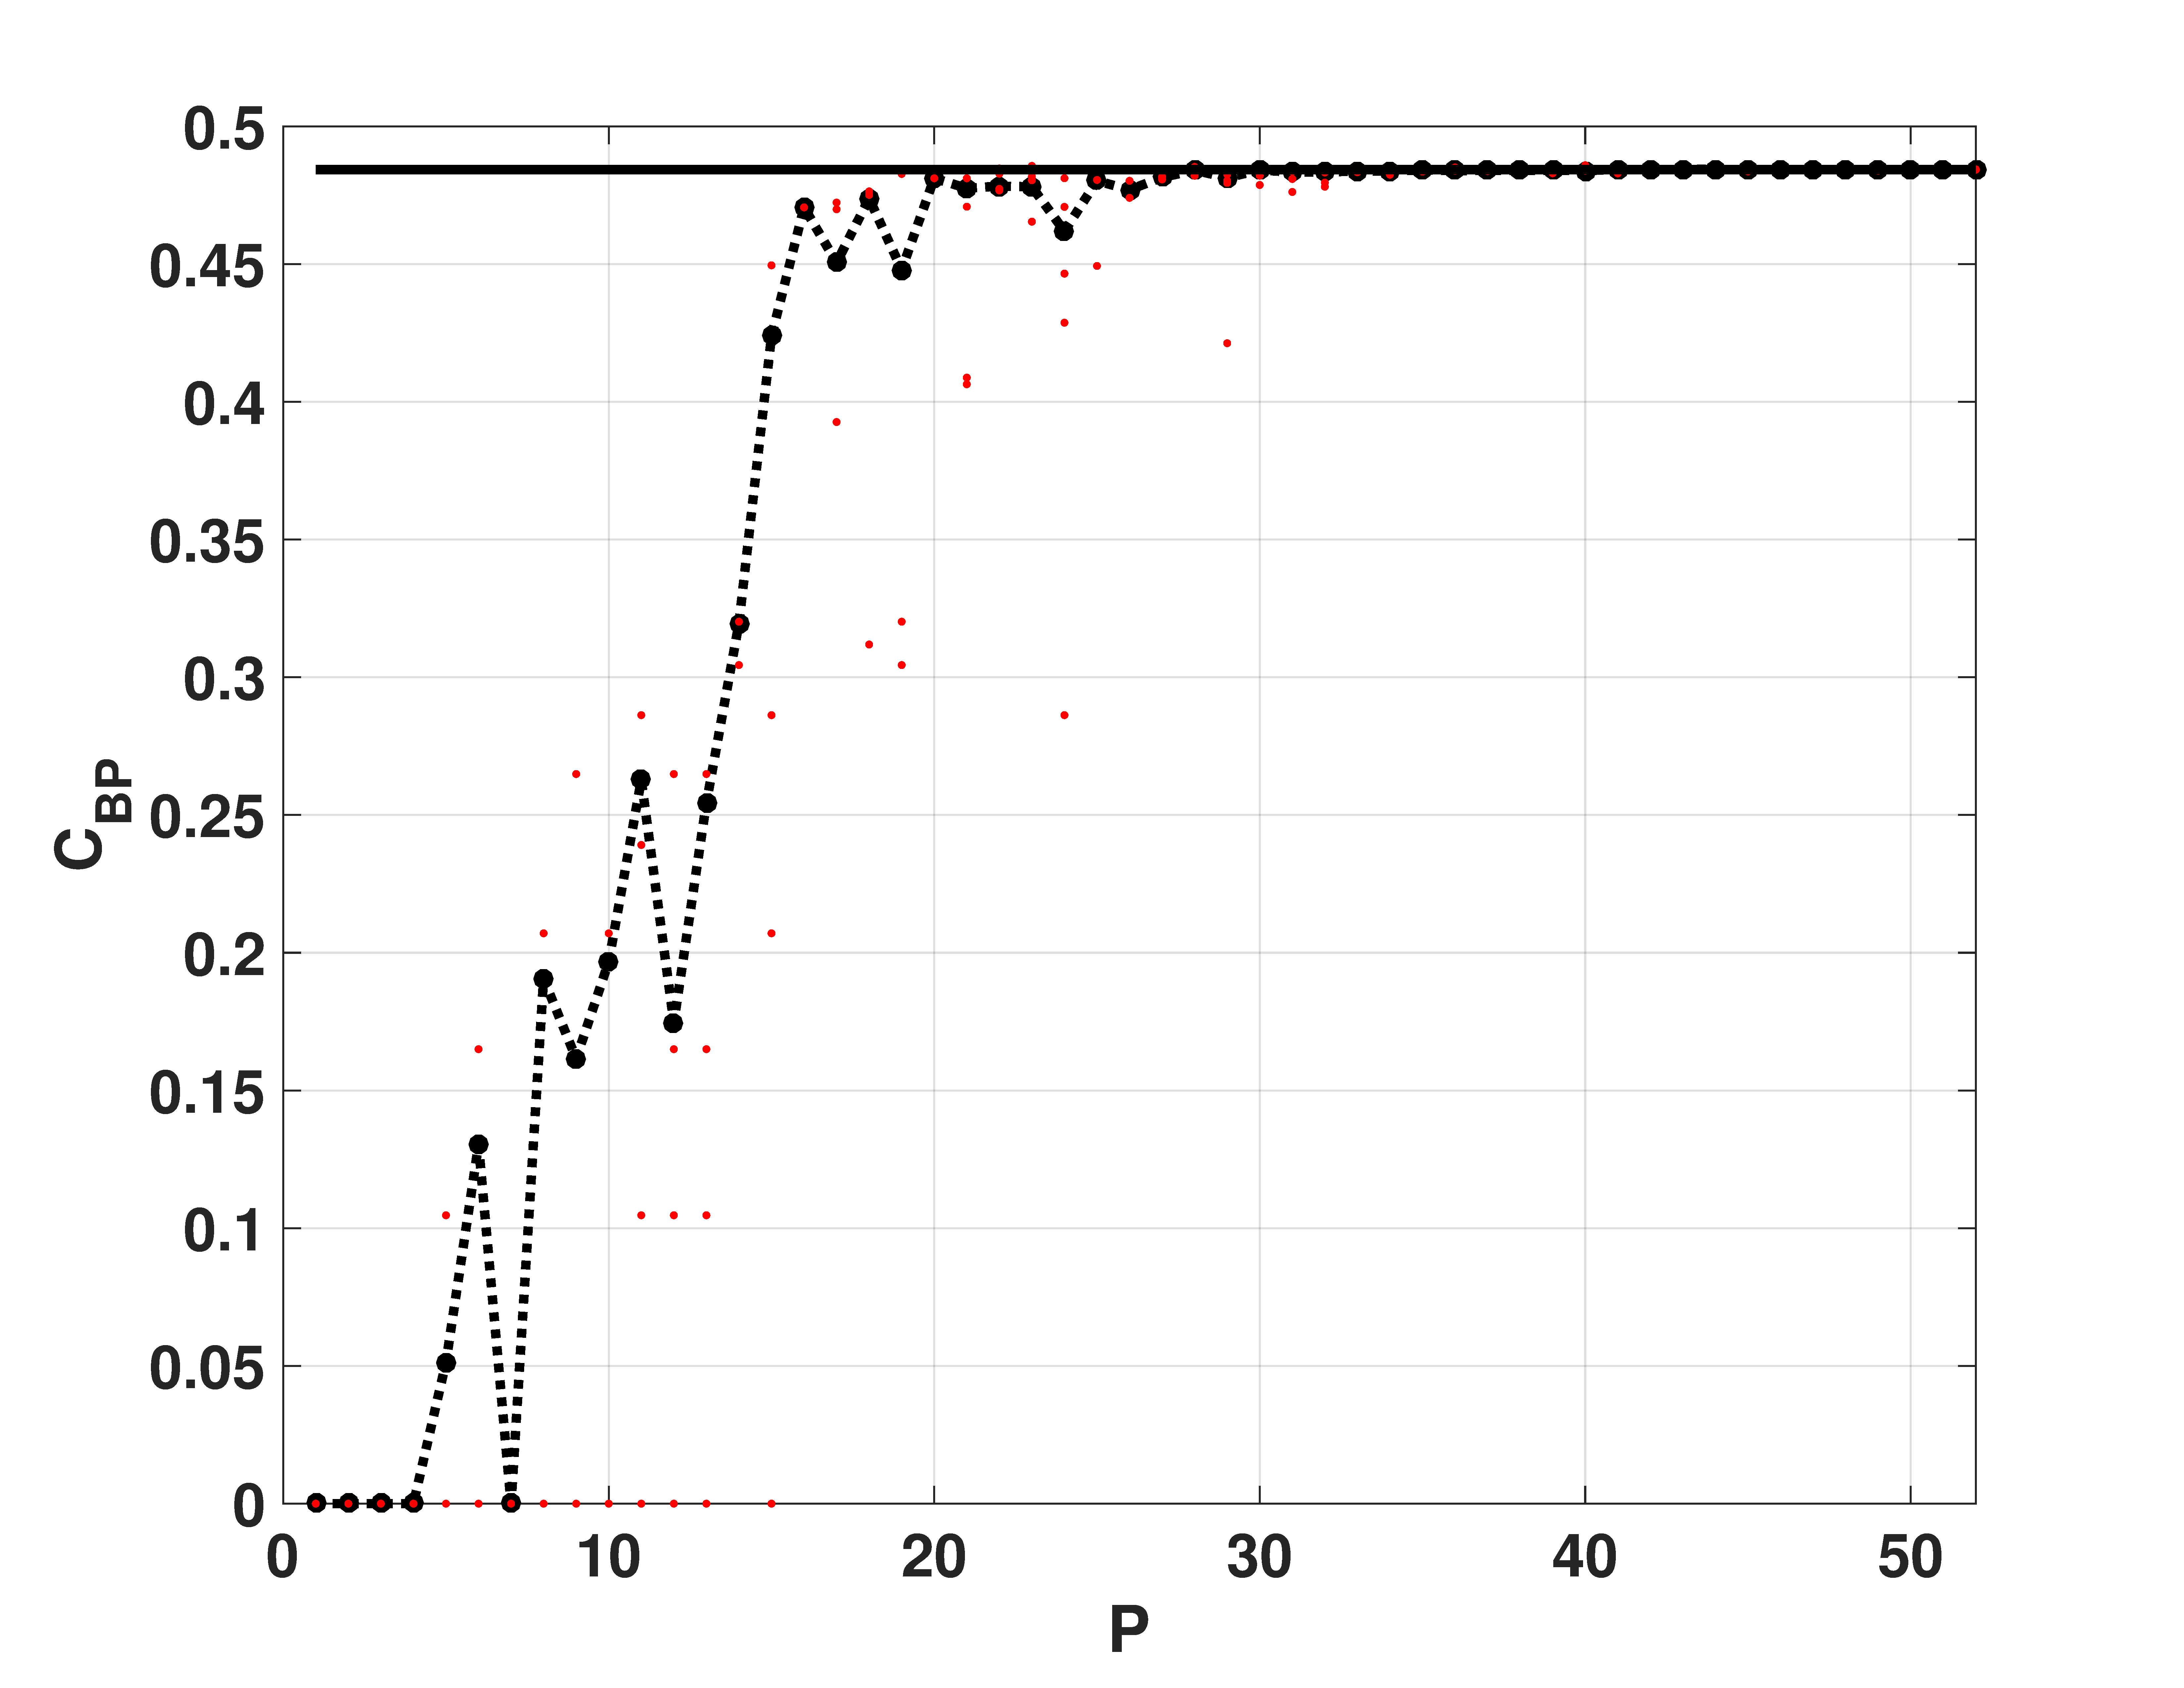
\includegraphics[width= .49\textwidth]{Cbp_Log}
	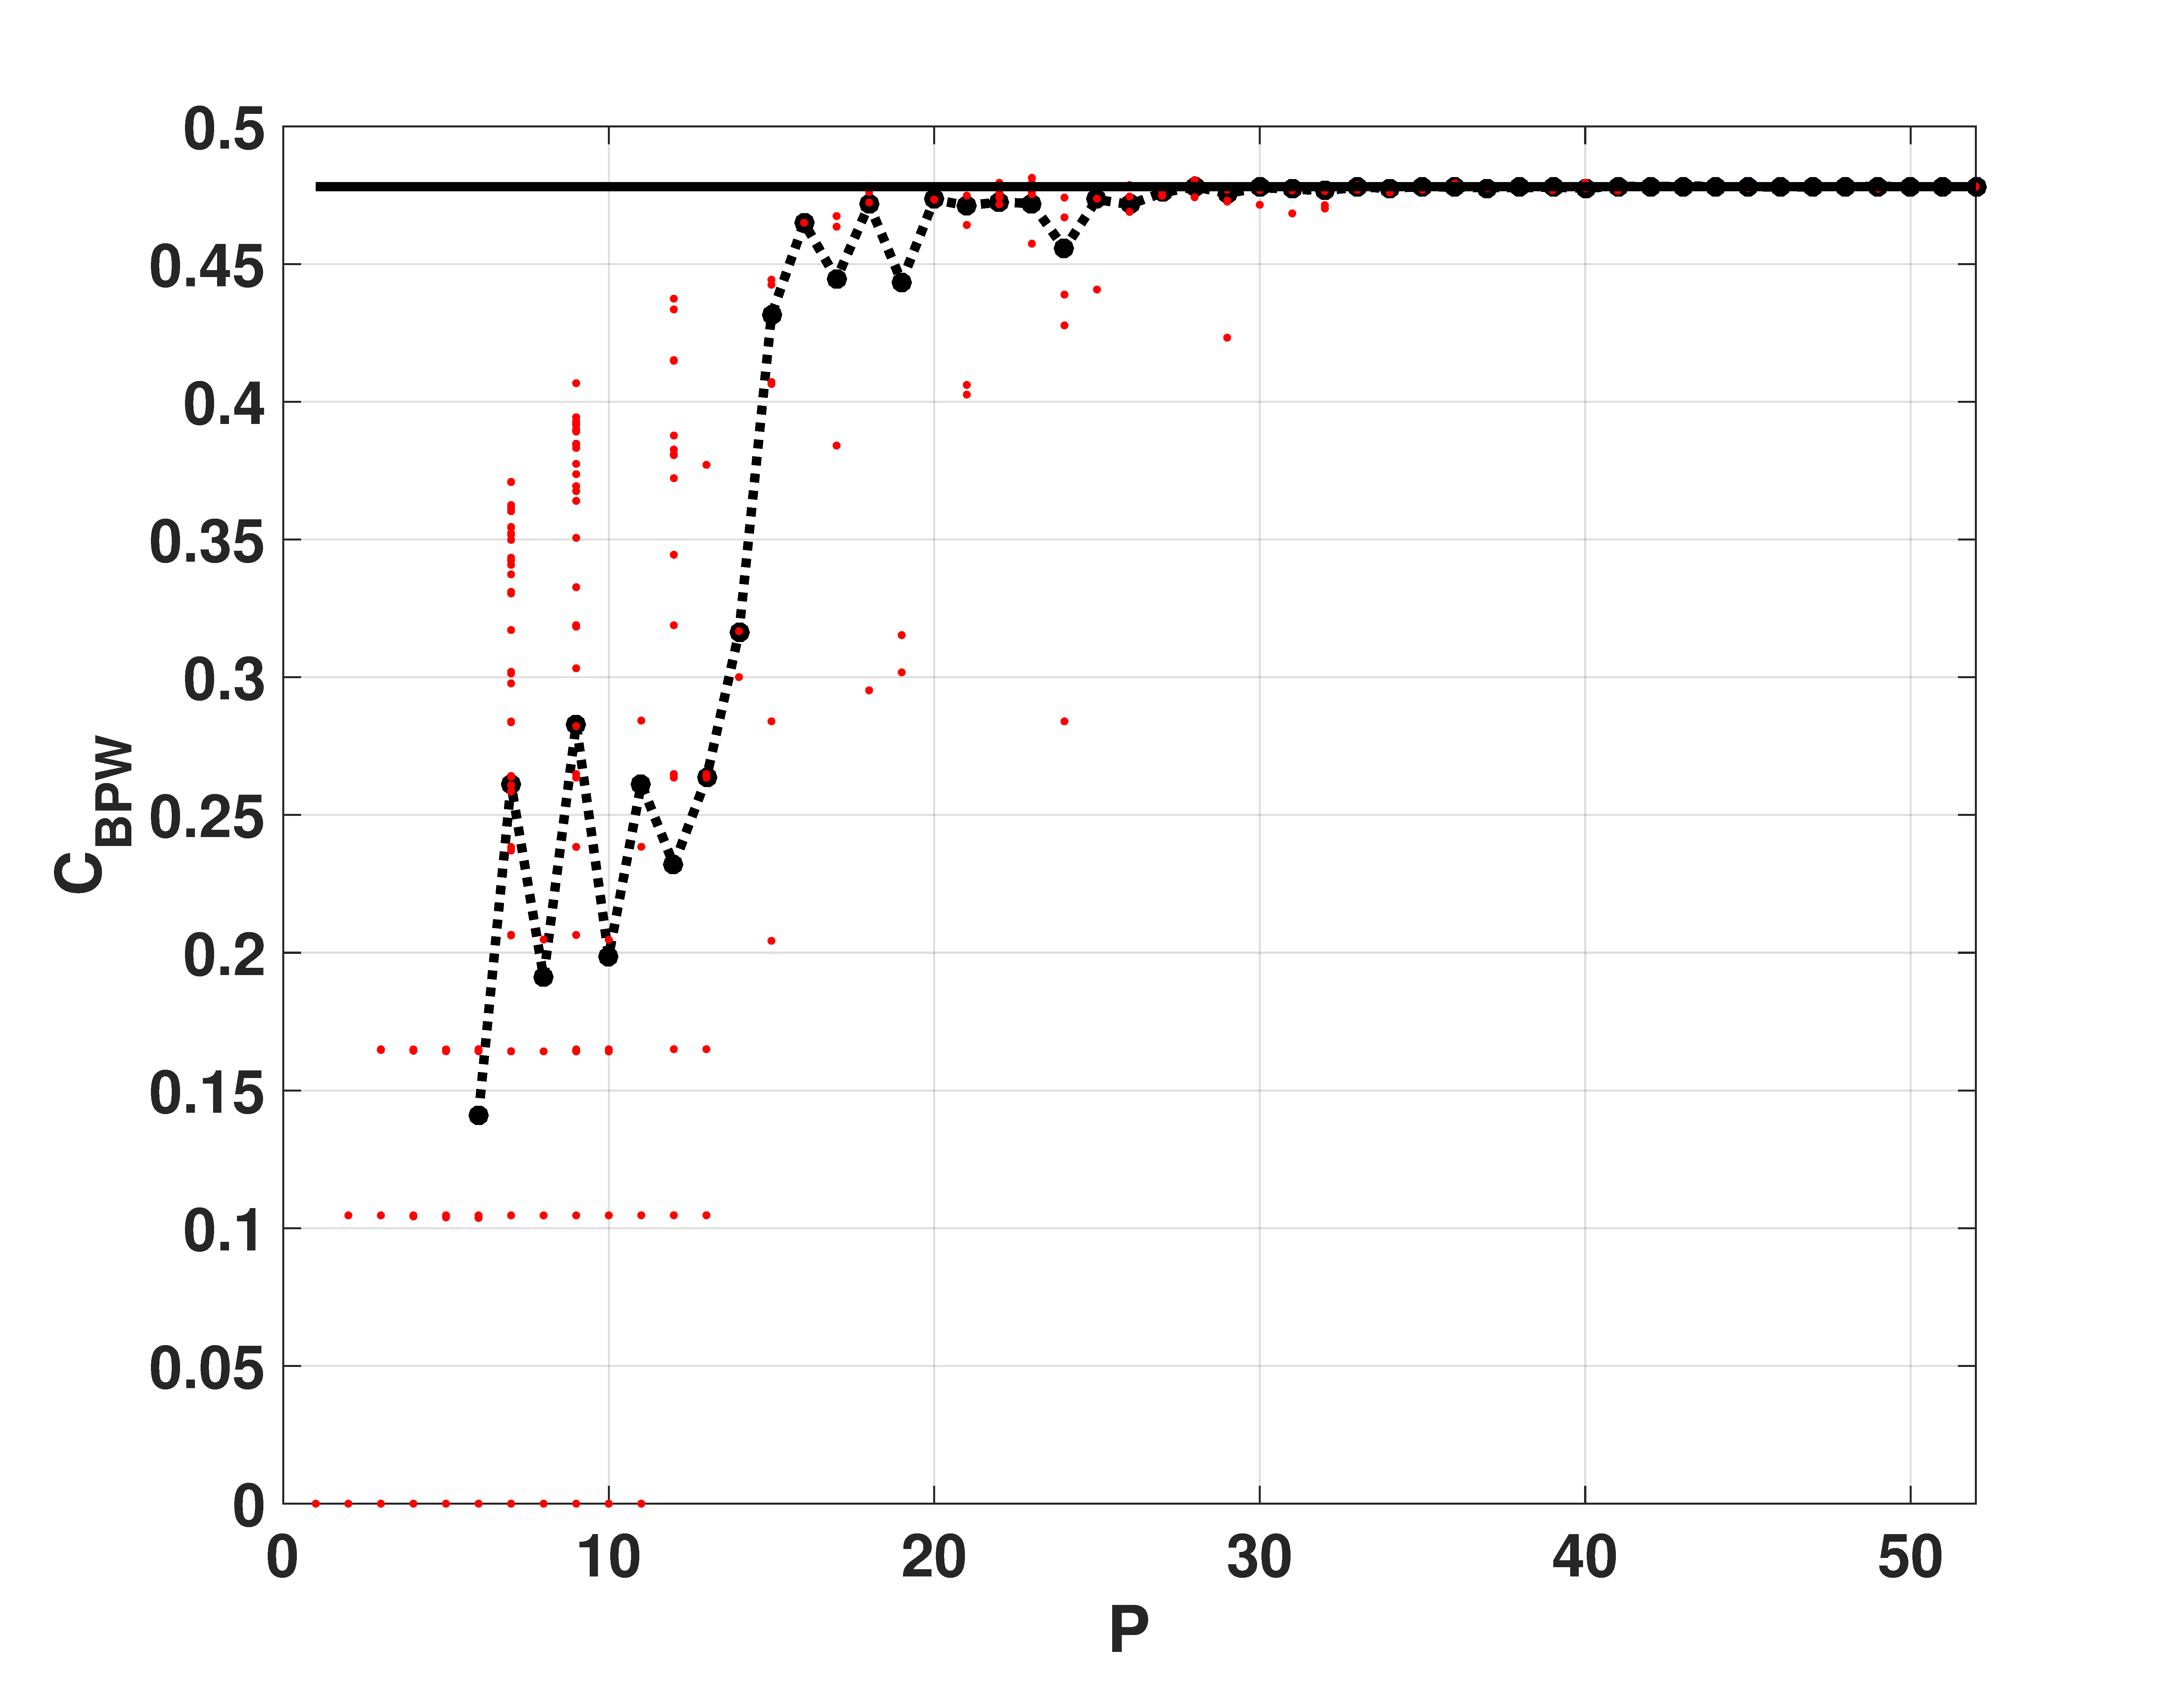
\includegraphics[width= .49\textwidth]{Cbpw_Log}
	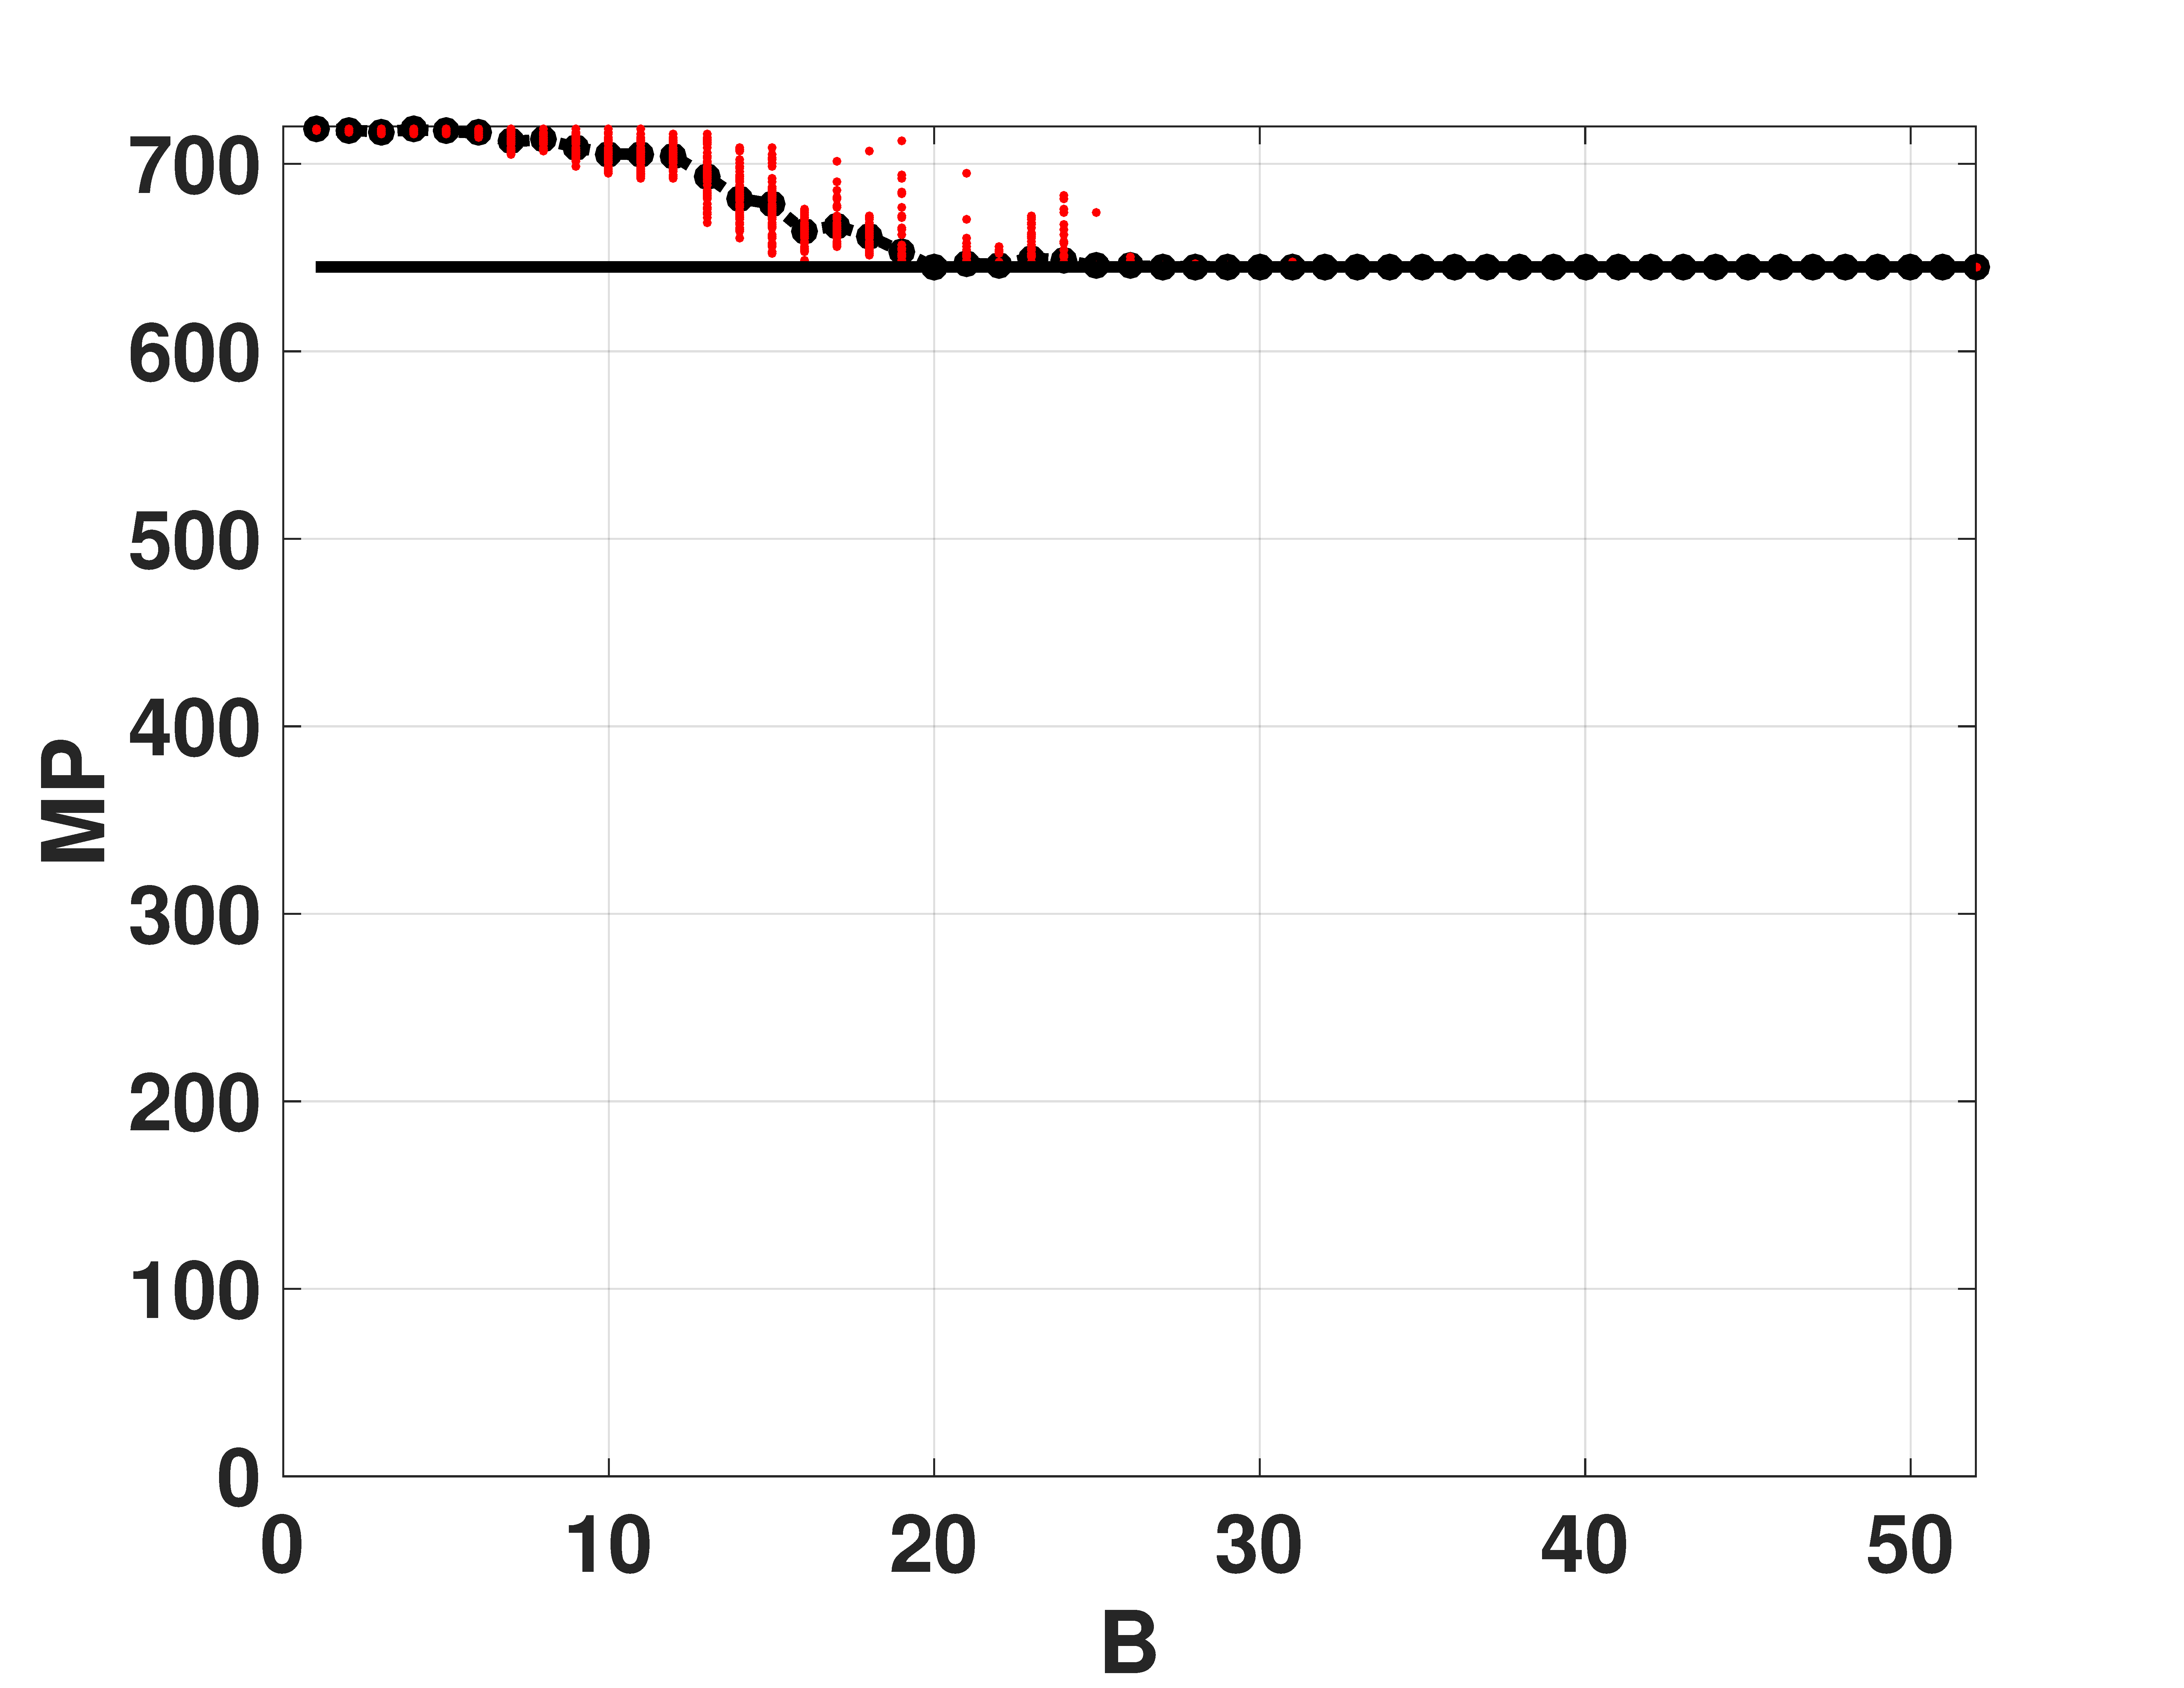
\includegraphics[width= .49\textwidth]{MP_Log}
	\caption{Statistical properties of the LOG map: (a) $H_{val}$ vs $B$ (b) $H_{BP}$ vs $B$ (c) $C_{BP}$ vs $B$ (d) $MP$ vs $B$.}
	\label{fig:LOG_QuantiB}
\end{figure}

The same results are now shown in double entropy planes with the precision as parameter (Fig. \ref{fig:LOG_HH}).
These figures show: $100$ red points for each fixed point precision ($B$) and in black their average (dashed black line connecting black dots), $100$ blue dots that are the results of each run in floating point and a black star their average.
This last $100$ points and their average are overlapped.

As expected, the fixed point architecture implementation converges to the floating point value as $B$ increases.
For both, Hbp-Hval and Hbpw-Hval, from $B=20$, $H_{val}$ improves but $H_{BP}$ remains constant.
It can be seen that the distribution of values reaches high values ($<H_{val}>=0.9669$) but their mixing is poor ($<H_{BP}>=0.6269$).

\begin{figure}
	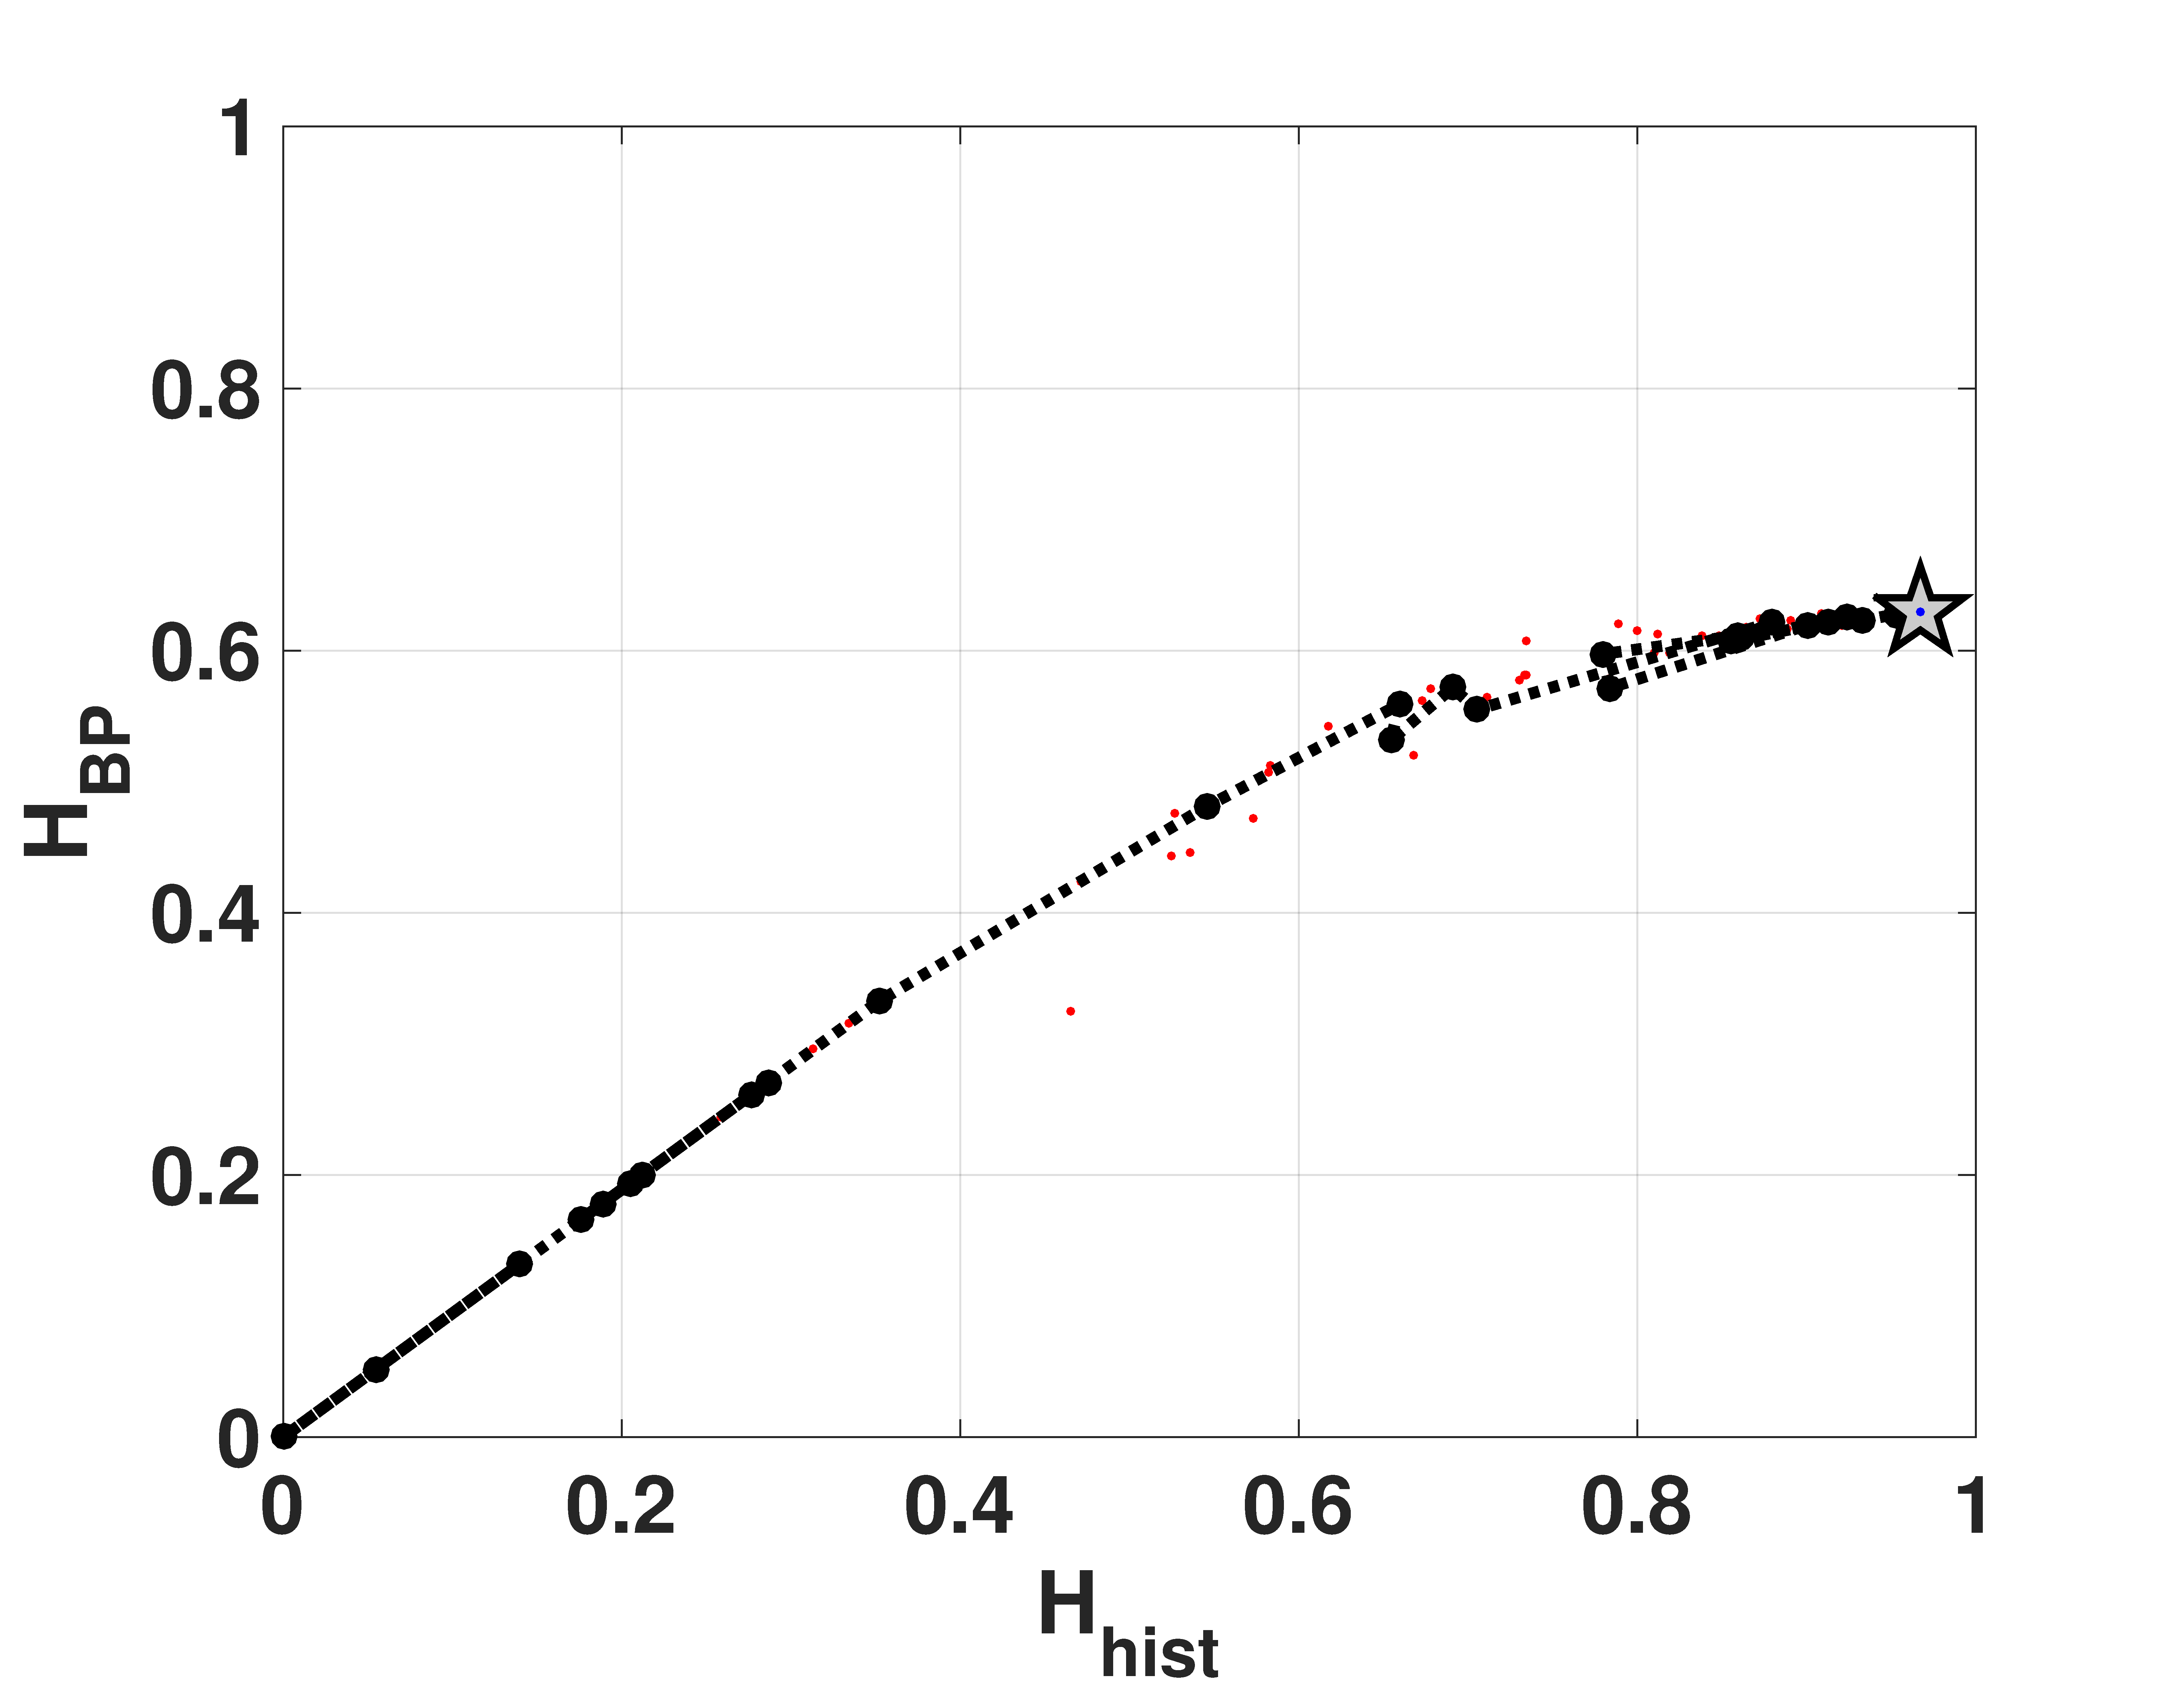
\includegraphics[width= .49\textwidth]{HbpHval_Log}
	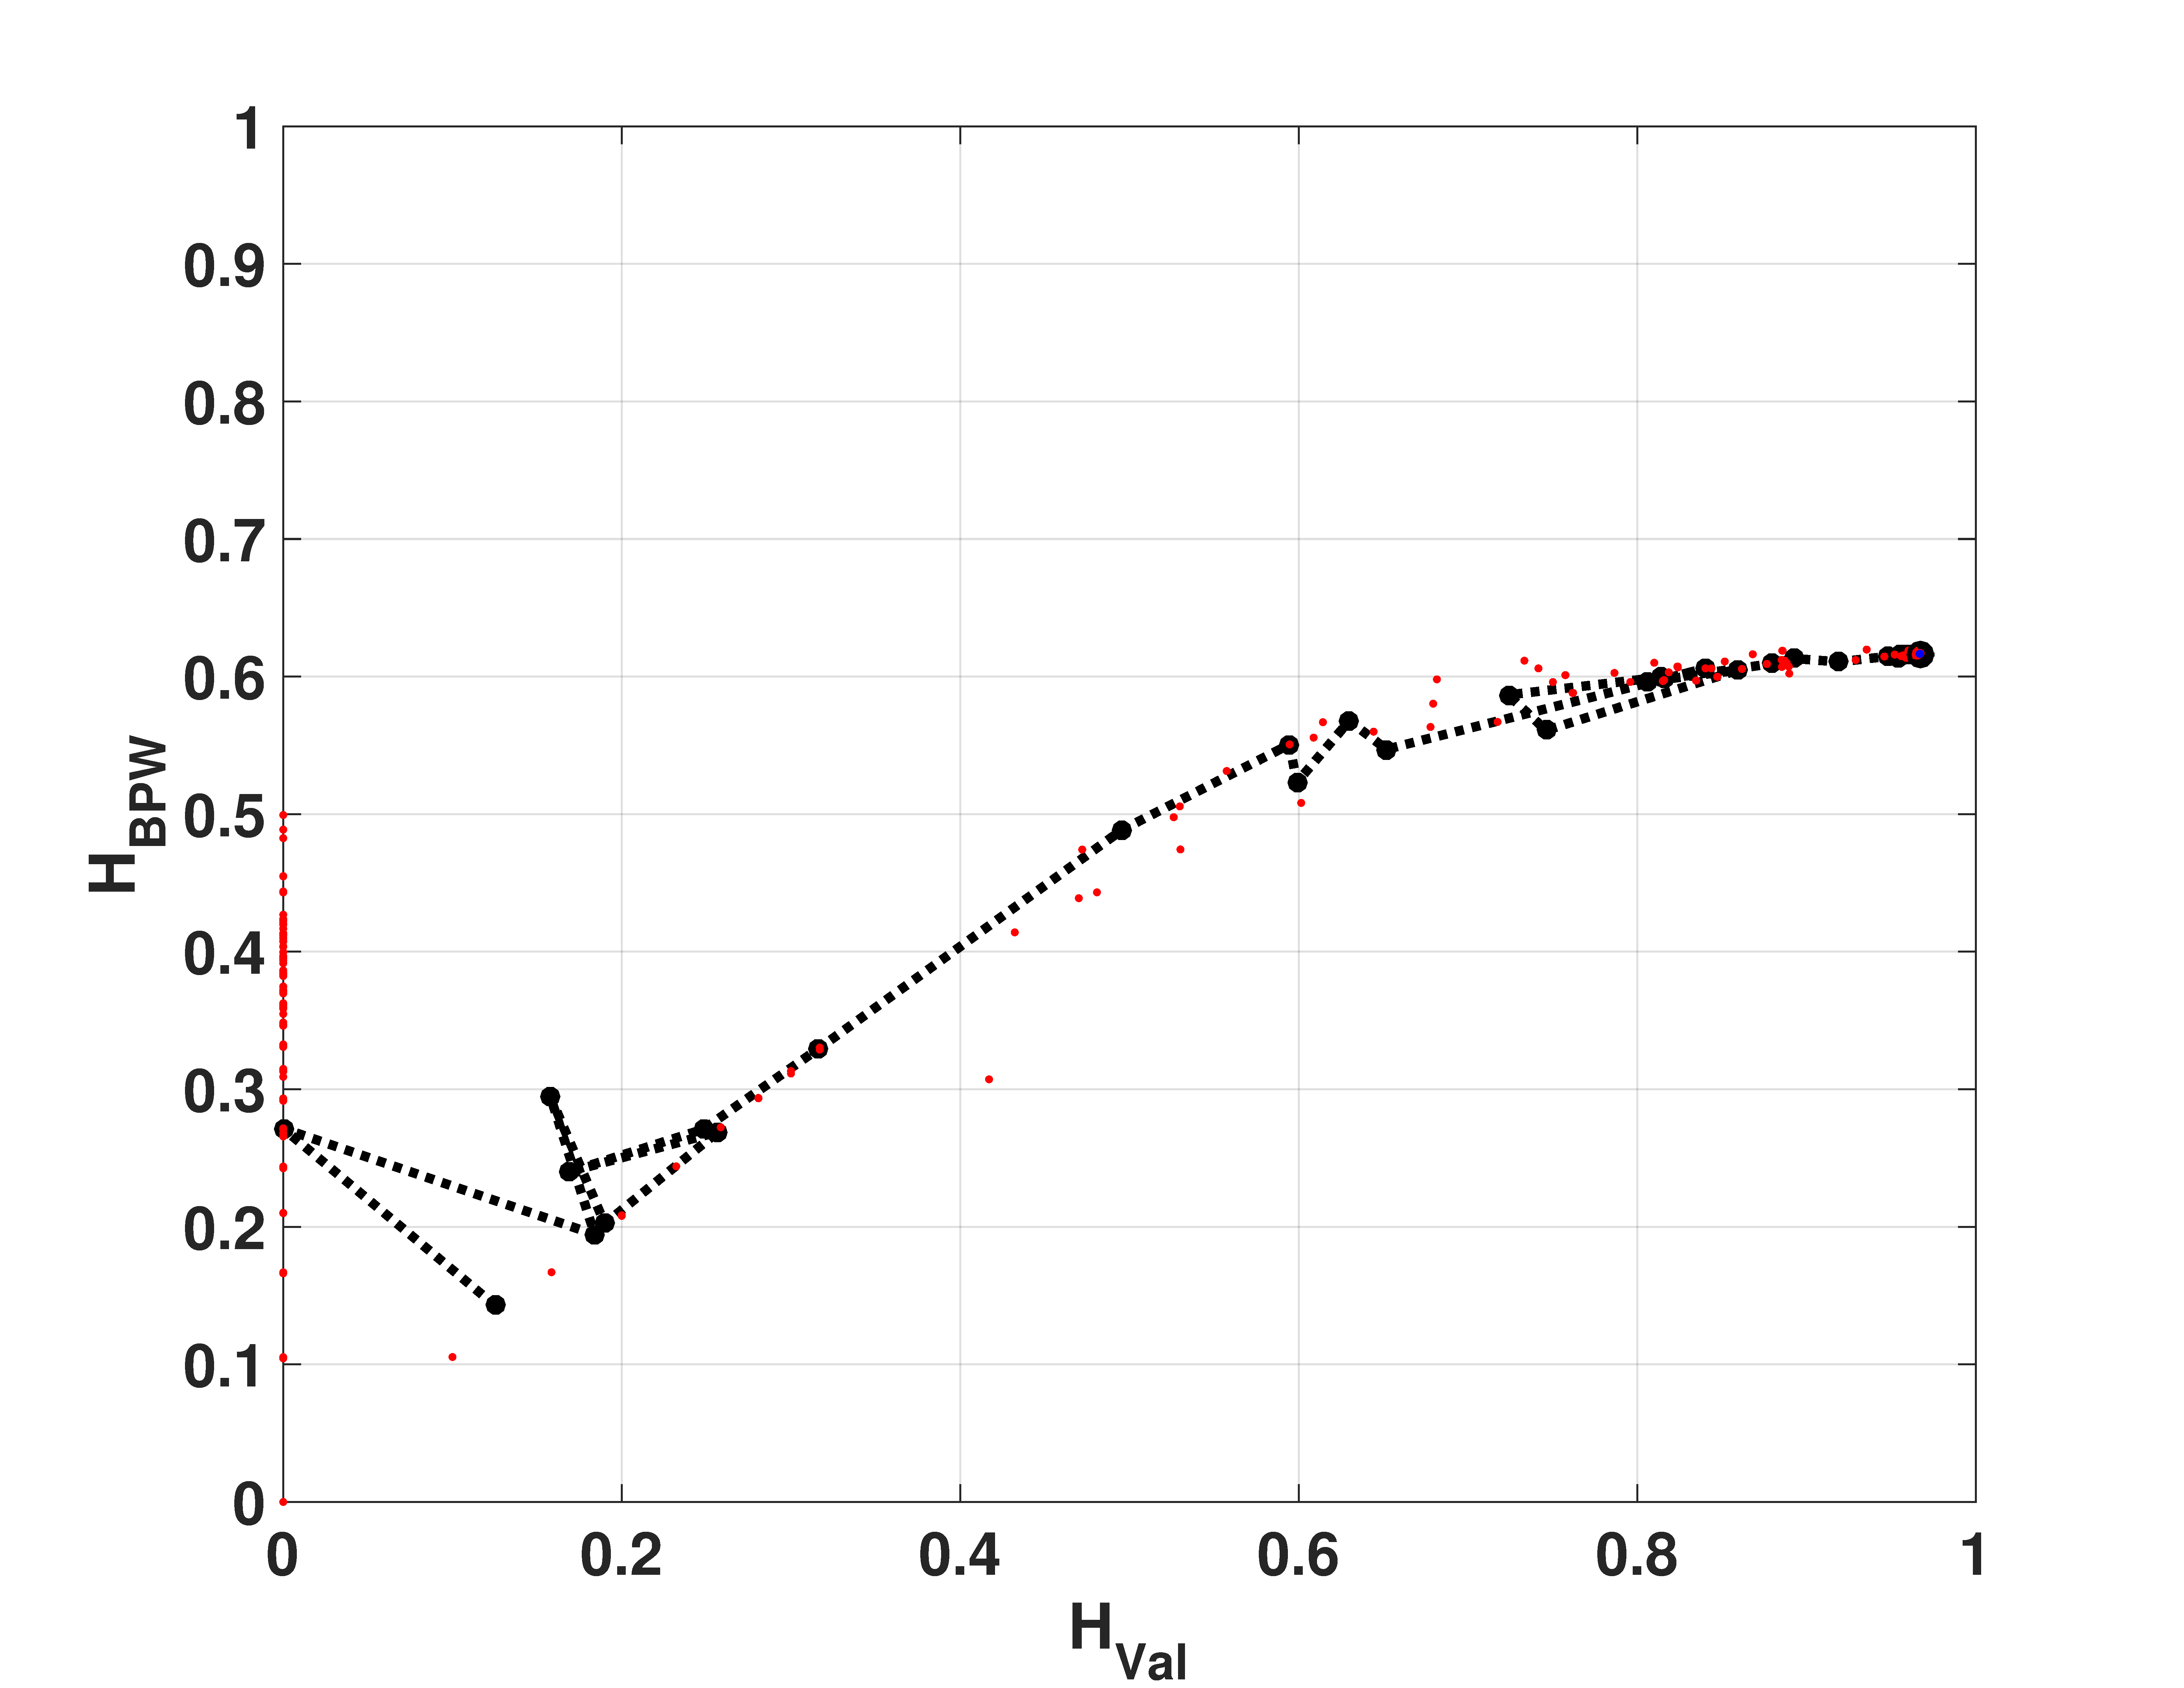
\includegraphics[width= .49\textwidth]{HbpwHval_Log}
	\caption{Evolution of statistical properties in double entropy plane of LOG map: (a) $H_{val}$ vs $H_{BP}$ (b) $H_{val}$ vs $H_{BPW}$.}
	\label{fig:LOG_HH}
\end{figure}

In Fig. \ref{fig:LOG_HC} we show the entropy-complexity planes.
Dotted gray lines are the upper and lower margins, is expected that a chaotic system remains near the upper margin.
These results characterize a chaotic behaviour, in $H_{BP}-C_{BP}$ plane we can see a low entropy and high complexity.

\begin{figure}
	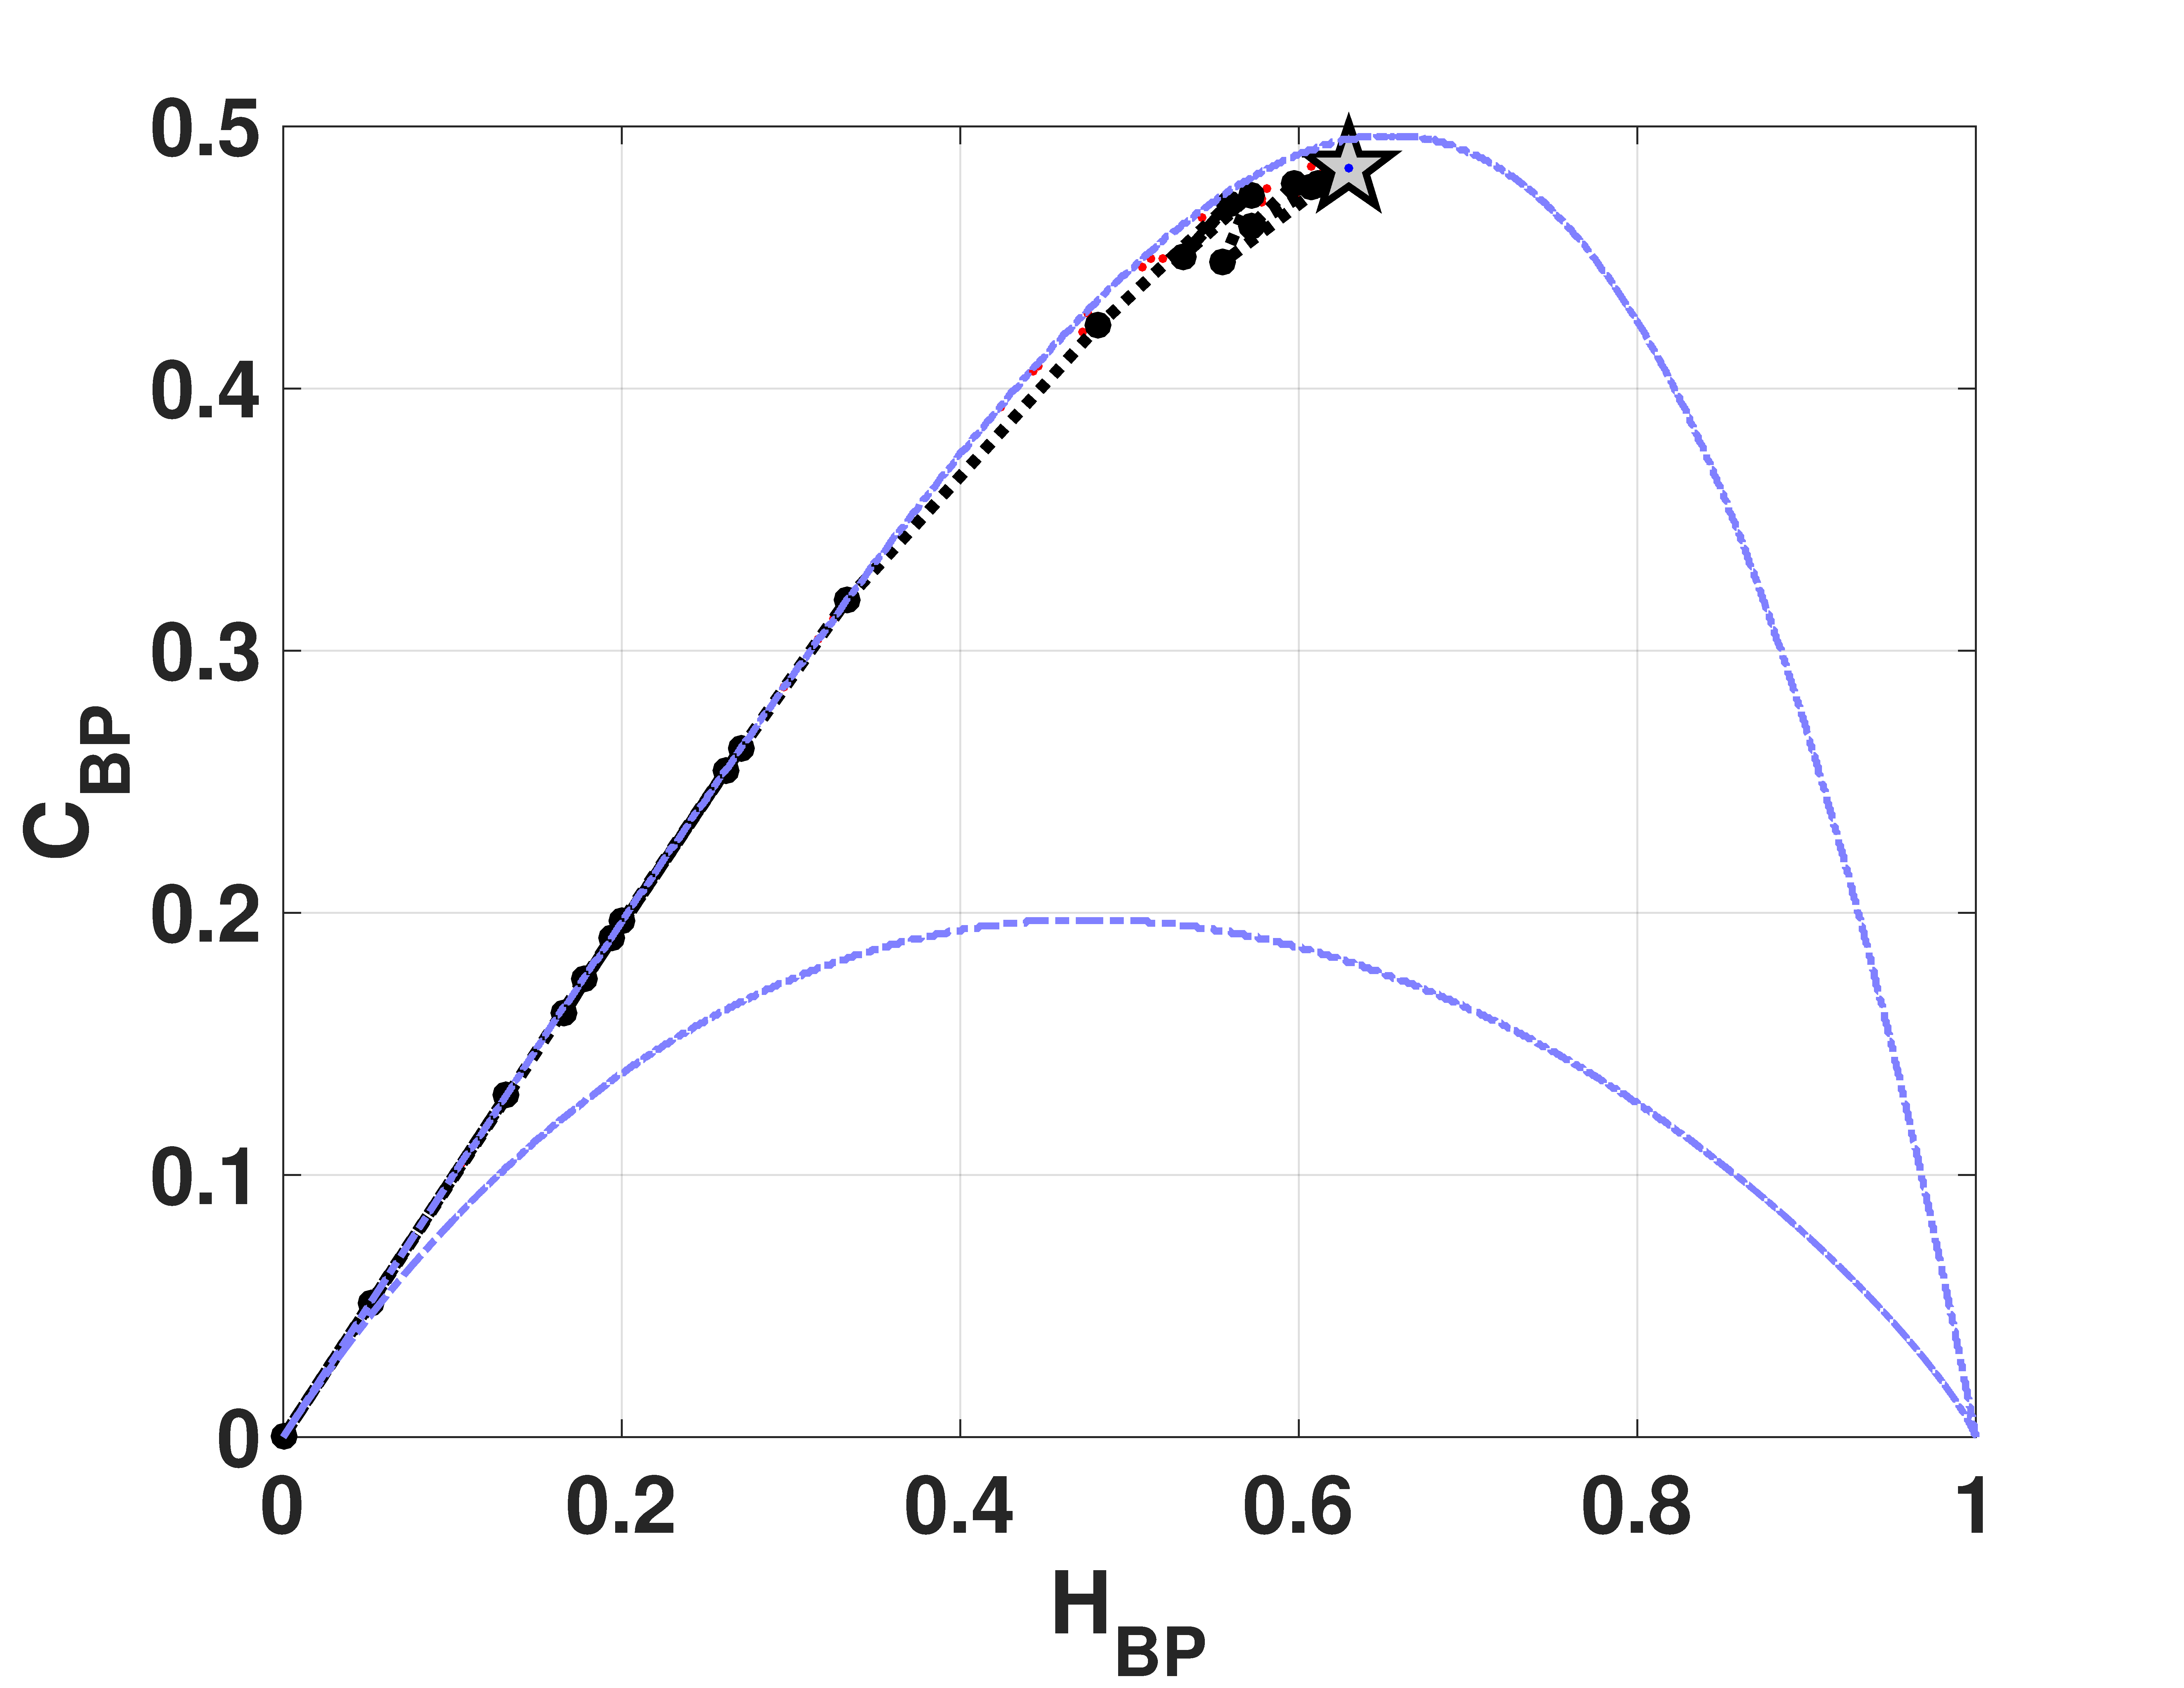
\includegraphics[width= .49\textwidth]{CbpHbp_Log}
	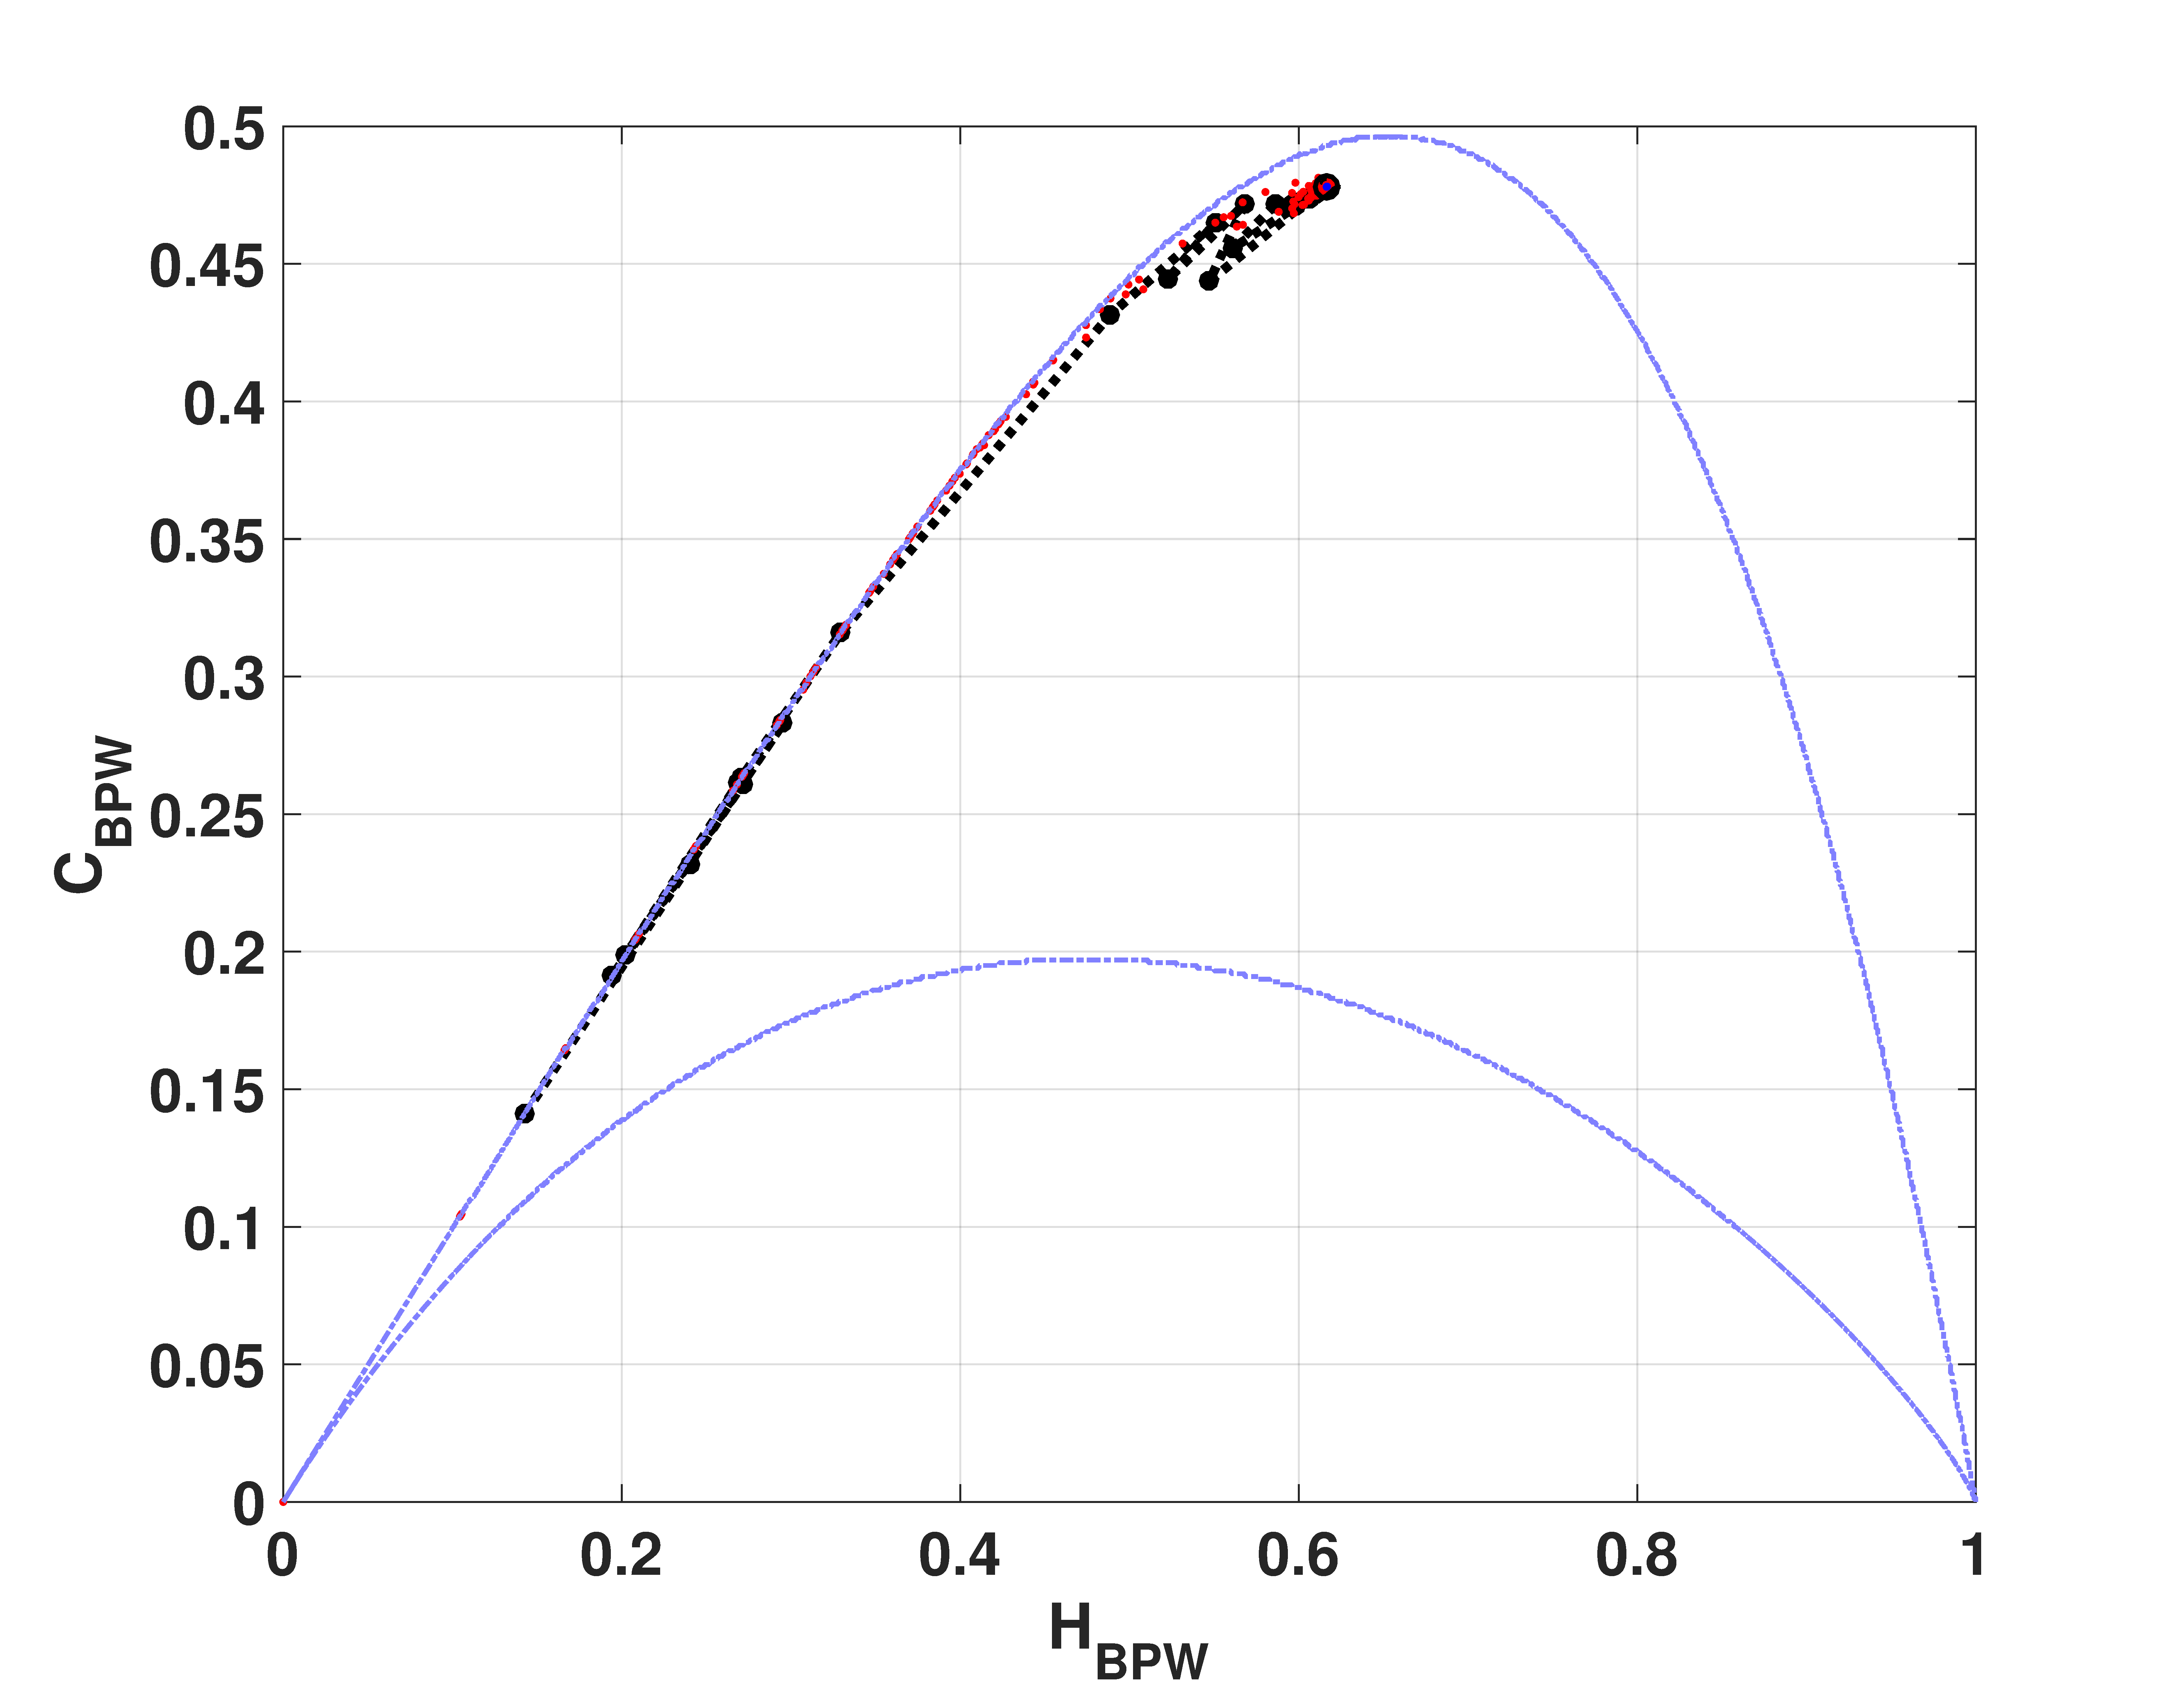
\includegraphics[width= .49\textwidth]{CbpwHbpw_Log}
	\caption{Evolution of statistical properties in entropy-complexity plane of LOG map: (a) $C_{BP}$ vs $H_{BP}$ (b) $C_{BPW}$ vs $H_{BPW}$.}
	\label{fig:LOG_HC}
\end{figure}
